% Información para el motor (arara). Compilar en LuaLaTeX o XeLaTeX sólamente.

%arara: lualatex: {
%arara: --> interaction: nonstopmode,
%arara: --> options: ['-file-line-error'],
%arara: --> shell: yes,
%arara: --> synctex: yes,
%arara: --> }
%arara: makeglossaries
%% arara: makeindex

\documentclass[letterpaper,twoside]{article}

 %%%%%%% VARIABLES ESTÁTICAS %%%%%%%
% Aqui se definen las variables para diferentes procedimientos.
% Verificar que las unidades coincidan si se deciden cambiar.

\newcommand{\defglo}[1]{\item[{\bfseries \glsname{#1}}] \glsdesc{#1}} % Define un comando para dar un item en un entorno de descripción para una palabra definida en el glosario
% \includeonly{src/PSA-2.19.tex,src/PSA-Gloss.tex}
\newcommand{\TipoID}{TEMP} % Definirlo como: PRO, PROG, ToC, G, L, CE, CI, I, etc.
\newcommand{\Prog}{TEMP}
\newcommand{\ProgTitulo}{TEMP}

\newcommand{\ie}{\emph{i.e.}}
\newcommand{\eg}{\emph{e.g.}}

%%%%%%%%%%%%%%%% Formularios %%%%%%%%%%%%%%%%
\newcommand{\IdFormAACC}{F-OP-40}

\newcommand{\BitES}{Bitácora de entradas y salidas --- Clientes (F-AD-1)}
\newcommand{\BitULl}{Bitácora de uso de llaves (F-AC-1)}
\newcommand{\BitVig}{Bitácora de vigilancia (F-AC-2)}
\newcommand{\Fpap}{Papeleta (F-AC-3)}
\newcommand{\Oent}{Orden de entrada (F-AC-4)}
\newcommand{\Osal}{Orden de salida (F-AC-5)}
\newcommand{\LayES}{Layout de carga o descarga (F-AC-6)}
\newcommand{\BitClor}{Bitácora de cloración de agua (F-AC-7)}
\newcommand{\BitTap}{Bitácora de concentración de tapete sanitario (F-AC-8)}
\newcommand{\BitUQ}{Bitácora de uso de productos químicos (F-AC-9)}
\newcommand{\BitLAd}{Bitácora de limpieza de aduana sanitaria (F-AC-10)}
\newcommand{\BitLOf}{Bitácora de limpieza de oficinas (F-AC-11)}
\newcommand{\BitLEx}{Bitácora de limpieza de exteriores (F-AC-12)}
\newcommand{\BitBPH}{Bitácora de cumplimiento de BPH (F-HyS-1)}
\newcommand{\BitCAP}{Bitácora de consumo de agua potable (F-HyS-2)}
\newcommand{\BitCE}{Bitácora de consumo de energía eléctrica (F-HyS-3)}
\newcommand{\BitIEx}{Bitácora de inspección de extintores (F-HyS-4)}
\newcommand{\BitVIR}{Bitácora de verificación de termómetros infrarrojos (F-HyS-5)}
\newcommand{\LVCMo}{Lista de verificación de condición de montacargas (F-HyS-6)}
\newcommand{\RTAC}{Registro de temperaturas con termómetro IR --- Aseguramiento de calidad (F-HyS-7)}
\newcommand{\RTMa}{Registro de temperaturas con termómetro IR --- Mantenimiento (F-HyS-8)}
\newcommand{\RAcL}{Registro de actividad de limpieza (F-HyS-9)}
\newcommand{\RAcM}{Registro de actividad de mantenimiento (F-Hys-10)}
\newcommand{\ReEq}{Registro de revisión de equipos de enfriamiento (F-MAN-1)}
\newcommand{\RCMi}{Registro de inspección de infraestructura en prevención (F-MAN-2)}
\newcommand{\Rcap}{Registro de asistencia a capacitación (F-MAN-3)}
\newcommand{\REvDQ}{Registro de eventos de derrame de químicos (F-MAN-4)}
\newcommand{\InvVyPD}{Registro de inventario de vidrio y plástico duro (F-MAN-5)}
\newcommand{\RVerSGC}{Registro de verificación del sistema de gestión de calidad (F-MAN-6)}
\newcommand{\RRCA}{Registro de recorrido de control de alérgenos (F-MC-1)}
\newcommand{\RAC}{Registro de acción correctiva o preventiva (F-OP-1)}
\newcommand{\RACQ}{Registro de acción correctiva --- Quejas (F-OP-2)}
\newcommand{\RVSCP}{Registro de verificación del servicio de control de plagas (F-OP-3)}
\newcommand{\RevD}{Registro de revisión diaria (F-SEG-1)}
\newcommand{\RCVyPD}{Registro de evento de contaminación por VyPD (F-SEG-2)}
\newcommand{\REvCA}{Registro de evento de contaminación por alérgeno (F-SEG-3)}



%%%%%%%%%%%%%%%% CÓDIGOS PSA %%%%%%%%%%%%%%%%
% \newcommand{\PSA}{PSA-3-PRO}                 % PSA-2.3 Inspección de producto durante su almacenamiento

%%%%%%%%%%%%%%%% PSA-2.3 | Inspección de producto durante su almacenamiento %%%%%%%%%%%%%%%%
\newcommand{\TiempoAndenCong}{\qty{\leq 30}{\minute}}
\newcommand{\TiempoAndenRefri}{\qty{\leq 30}{\minute}}
\newcommand{\TiempoAveriaRefri}{4}              % Tiempo máximo de permanencia de alimento refrigerado en cámara averiada (en horas) 
\newcommand{\TiempoAveriaConge}{10}             % Tiempo máximo de permanencia de alimento congelado en cámara averiada (en horas)
\newcommand{\EspacioMinimoParedProducto}{30}    % Espacio entre tarima y pared (en centimetros)
\newcommand{\EspacioMinimoTechoProducto}{30}    % Espacio entre tarima y techo (en centimetros)
\newcommand{\VecesTempManual}{dos}              % Veces que se verifica la temperatura manualmente



%%%%%%%%%%%%%%%% PSA-2.3 | Política de aprobación de proveedores %%%%%%%%%%%%%%%%
\newcommand{\NotifAuditoriaAProveedor}{2 semanas}           % Plazo máximo para notificar a proveedor sobre auditoría.
\newcommand{\PlazoResultadoAProveedor}{2 semanas}           % Plazo máximo para notificar a proveedor sobre resultados de auditoría.
\newcommand{\PlazoPlanDeAccionAuditProveedor}{2 semanas}    % Plazo maximo para recibir plan de acción de parte del proveedor tras auditoría

%%%%%%%%%%%%%%%% PSA-2.15 | Almacenamiento de registros %%%%%%%%%%%%%%%%
\newcommand{\VigenciaAlmacRegistros}{2 años}
\newcommand{\VigenciaAlmacRegistrosElec}{3 años}

%%%%%%%%%%%%%%%% GLOBAL | Resetear glosarios en cada sección %%%%%%%%%%%%%%%%
\usepackage{etoolbox}
\preto\section{\glsresetall}

\newcommand{\AC}{aseguramiento de calidad}
\newcommand{\G}{gerencia}
\newcommand{\AD}{alta dirección}
\newcommand{\OP}{operaciones}
\newcommand{\Emb}{embarques}
\newcommand{\MC}{mesa de control}     % Definición de variables estáticas
                                        % i.e. Tiempo máximo de cámras de refrigeración sin energía



%%%%%%%%%%%%%%%%%%%%%%%%%%% ESPECIALES %%%%%%%%%%%%%%%%%%%%%%%%%%%%%%%%%%
% \RequirePackage{expl3}    % \usepackage cannot be used before \documentclass
% \ExplSyntaxOn             % Switch on expl3 syntax
% \pdf_version_gset:n{1.7}  % Use provided expl3 function
% \ExplSyntaxOff            % Switch off expl3 syntax

%%%%%%%%%%%%%%%%%%%%%%%%%%% Tipografía %%%%%%%%%%%%%%%%%%%%%%%%%%%%%%%%%%

\usepackage[sfdefault,t,lf]{carlito}    % Alternativa OpenSource a Calibri, definir sans serif como predeterminado, numerales tabulares
% \usepackage[default,lnum]{opensans}
% \usepackage{CormorantGaramond}

% \usepackage{lucidabr}

% \usepackage{fontspec}

\fontsize{8.8pt}{12pt}\selectfont
\renewcommand{\baselinestretch}{1.2}

% \linespread{1.3}
% \DeclareUnicodeCharacter{2212}{-}

\usepackage{polyglossia}
	\setdefaultlanguage[spanishoperators=all]{spanish}  % Definir la localización del documento como es-MX (para que cuadro sea tabla, etc.)
	% \setdefaultlanguage{mexican}
	\renewcommand{\listtablename}{Índice de tablas}

\usepackage{changelog}  % Control de versiones
\usepackage{float}
\usepackage{pdflscape}
\usepackage{pifont}
\newcommand{\cmark}{\ding{51}}%
\newcommand{\xmark}{\ding{55}}%

\usepackage[%
toc=true,
postpunc={;},
acronyms,
xindy]{glossaries-extra}    % Manager de glosarios, usar xindy para el indice alfabético
% \usepackage{glossary-mcols}
% \renewcommand{\glsmcols}{2}
\setglossarystyle{long3col}

	\makeglossaries{}
	% \setabbreviationstyle[acronym]{short-long}  % Estilo de acrónimos
	\setabbreviationstyle[acronym]{long-short}
	% \setglossarystyle{mcolindex}
	\loadglsentries[main]{../glosario-def.tex}  % Archvio que LuaLaTeX toma para las definiciones

	\renewcommand{\glossarypreamble}{\fontsize{10pt}{12pt}\selectfont}

	
\usepackage{imakeidx}       % Para hacer indices
	\makeindex[columns=2]   % Estilo del indice alfabético

\newcounter{note}[section]  % Nuevo contador para notas
\renewcommand{\thenote}{\thesection.\Alph{note}}    % Definir estilo de numeración de las notas
\usepackage[framemethod=TikZ]{mdframed}             % Motor gráfico para notas (TikZ)
\newenvironment{note}[1][]{%                        % Nuevo entorno de Nota (note) 
    \refstepcounter{note}
    \begin{mdframed}[%                                  
        frametitle={Nota \thenote\ #1},                 % Titulo de las notas
        skipabove=\baselineskip{} plus 2pt minus 1pt,     % Espaciado superior
        skipbelow=\baselineskip{} plus 2pt minus 1pt,     % Espaciado inferior
        linewidth=0.5pt,                                % Tamaño de linea del recuadro
        frametitlerule=true,                            % incluir titulo
        frametitlebackgroundcolor=gray!30               % Color del recuadro
    ]%
}{%
    \end{mdframed}
}

\newcounter{contact}[section]                           % Nuevo contador para contactos
\renewcommand{\thecontact}{\thesection.\Alph{contact}}  % Definir que la numeración sea Sección.Alfabético

\newenvironment{contact}[1][]{%
    \refstepcounter{contact}
    \begin{mdframed}[%
        frametitle={Contacto \thecontact\ #1},          % Titulo del contacto
        skipabove=\baselineskip{}plus 2pt minus 1pt,     % Espaciado superior
        skipbelow=\baselineskip{}plus 2pt minus 1pt,     % Espaciado inferior
        linewidth=0.5pt,                                % Tamaño de linea del recuadro
        frametitlerule=true,                            % poner titulo
        frametitlebackgroundcolor=yellow!30             % Color del recuadro
    ]%
}{%
    \end{mdframed}
}

\usepackage[multiple]{footmisc}     % Cambios en la presentación de pies de página
\usepackage{microtype}              % Ajustes de kerning y otros 
\usepackage{graphicx}               % Mejora al motor de imagenes
\usepackage{hyperref}               % Referencias cruzadas en PDF
\usepackage{cleveref}               % Referencias cruzadas en texto
%%%%%% REDEFINICIONES DE REFERENCIAS CRUZADAS %%%%%%%%%
    \crefname{note}{nota}{notas}    
	\Crefname{note}{Nota}{Notas}
	\crefname{contact}{contacto}{contactos}
	\Crefname{contact}{Contacto}{Contactos}
	\crefname{paragraph}{parrafo}{parrafos}
	\Crefname{paragraph}{Parrafo}{Parrafos}
%%%%%%%%%%%%%%%%%%%%%%%%%%%%%%%%%%%%%%%%%%%%%%%%%%%%%%%
\newcommand{\email}[1]{\href{mailto:#1}{#1}}    % Comando para hacer que se puedan clickear emails
\newcommand{\cels}[1]{\qty{#1}{\celsius}}       % Escrir celsius rapido

\usepackage{lastpage}   % Definir variable para el numero total de páginas
\usepackage{siunitx}    % Unidades internacionales y alineamiento de decimales en tablas
	\sisetup{detect-all}    % Detectar automaticamente que la tipografía es sans serif

\usepackage{color}  % definir colores nuevos

\usepackage{tabularray} % Creación de tablas
	\UseTblrLibrary{booktabs,siunitx}   % librerias parea tablas correctas, unidades internacionales
	\definecolor{Gallery}{rgb}{0.929,0.929,0.929}   % definición del color "Gallery"
	\DefTblrTemplate{contfoot-text}{normal}{\textit{Continúa en la siguiente página}}   % Continuación de tabla
	\SetTblrTemplate{contfoot-text}{normal} % Continuación de tabla normal (footer)
	\DefTblrTemplate{conthead-text}{normal}{\textit{(Continuación)}}    % Continuación de tabla
	\SetTblrTemplate{conthead-text}{normal} % Continuación de tabla (header)

    % \usepackage[margin=1cm,bmargin=2cm,tmargin=5cm,headheight=110pt]{geometry}   % Dispoción espacial del documento
% \newgeometry{includeheadfoot, heightrounded, left=1cm, right=1cm, top=1cm, bottom=4cm, headheight=6em, footskip=1.5em}    
%     \savegeometry{L1}

% \newgeometry{includeheadfoot, heightrounded, left=1cm, right=1cm, top=1cm, bottom=4.5cm, headheight=7em, footskip=1.5em, showcrop, showframe}
%     \savegeometry{L2}

\usepackage[%
includeheadfoot,
heightrounded,
left=1cm,
right=1cm,
top=1cm,
bottom=1cm,
headheight=110pt,
footskip=1.5em]{geometry}    

\usepackage[export]{adjustbox}

\usepackage{enumitem}
	\setlist[1]{labelindent=\parindent} % Indentación como parrafo para listas
	\setlist[description]{style=nextline}
	\setlist[itemize]{leftmargin=*} 	% Eliminar margen en izq
	\setlist[itemize,1]{label=---}  	% Viñeta como em-dash
	\setlist[itemize,2]{label=--}
	\setlist{noitemsep} 				% Que no se separen los item
	% [label={\theparagraph--\arabic*}] % Numerarar parrafo-numero

	\newlist{ListaSec}{enumerate}{3}
	\setlist[ListaSec]{label* = \arabic*., name* = \arabic{section}.\arabic{subsection}}


%%%%%%%%%%%%%%%% DEFINICIÓN DE CABECERA %%%%%%%%%%%%%%%%
\usepackage{fancyhdr}   % Usar fancy headers y footers
	\renewcommand{\headrulewidth}{0pt}  % Grosor de regla del header
	\fancyhead[CE,CO,LE,LO,RE,RO]{} % Resetear headers    
    \fancyfoot[CE,CO,LE,LO,RE,RO]{} % Resetear footers

%%%%%%%%%%%%%%%%%%%%%% VARIABLES DE CADA DOCUMENTO DENTRO DE UN PROGRAMA %%%%%%%%%%%%%%%%%%%%%
	\newcommand{\Codigo}{}                  % Codigo del documento
	\newcommand{\FechaPub}{}                % Fecha de publicación
	\newcommand{\Titulo}{}                  % Titulo del documento
	\newcommand{\MayorVer}{}                % Versión mayor
	\newcommand{\MenorVer}{}                % Verisón menor
	\newcommand{\Edit}{\MayorVer.\MenorVer} % Definición de la edición

    \newcommand{\Elaboro}{}                 % Nombre de quien lo elaboró
    \newcommand{\Reviso}{}                  % Nombre de quien revisó el documento
    \newcommand{\Autorizo}{}                % Nombre de quien aprobó el documento

%%%%%%%%%%%%%%%%%% Formato por defecto para informaicón documentada general %%%%%%%%%%%%%%%%%%
\fancypagestyle{formato-PS}{%
	\fancyhead{}
	\fancyfoot{}
	\fancyhead[RE]{%
		\begin{tblr}{%	
			colspec = {X[c,m]X[c,m]},    % Especificación de columnas: Anchura estática, centrado en medio
			hlines,
			vlines,
			width = 0.35\linewidth,}%
			{\textbf{Código:}\\ \Codigo} 				 & {\textbf{Edición:}\\ \MayorVer.\MenorVer} 			\\ 	% Logotipo (2 columnas), red de frios (3 columnas), código del documento
			{\textbf{Fecha de publicación:}\\ \FechaPub} & {Página~\thepage~de~\pageref{LastPage}} 		% Titulo (4 columnas), Fecha, edición
		\end{tblr}
	}%

	\fancyhead[LO]{%
		\begin{tblr}{%	
			colspec = {X[c,m]X[c,m]},   % Especificación de columnas: Anchura estática, centrado en medio
			hlines,
			vlines,
			width = 0.35\linewidth,}%
			{\textbf{Código:}\\ \Codigo} 					& {\textbf{Edición:}\\ \MayorVer.\MenorVer} 			\\	% Logotipo (2 columnas), red de frios (3 columnas), código del documento
			{\textbf{Fecha de publicación:}\\\FechaPub}	& {Página~\thepage~de~\pageref{LastPage}} 		% Titulo (4 columnas), Fecha, edición
		\end{tblr}
	}%

	\fancyfoot[C]{Página~\thepage~de~\pageref{LastPage}}   % Para que muestre Página # de #
	\fancyfoot[L]{\textbf{CONFIDENCIAL}}                    % CONFIDENCIAL
	\fancyfoot[R]{\Codigo~v.\Edit}                          % Estructura del código CODIGO v.EDICION
}%

\fancypagestyle{formato-PI}{%
	\fancyhead{}
	\fancyfoot{}
    \fancyhead[C]{%
	    \begin{tblr}{%	
            colspec = {X[c,m]X[c,m]X[c,m]X[c,m]X[c,m]X[c,m]},    % Especificación de columnas: Anchura estática, centrado en medio
            hlines,
            vlines,
			width = \linewidth,}%
			\SetCell[c=2]{} 
\includegraphics[height=3em, valign=c]{../RDF_Logo.png}	&	& \SetCell[c=3]{} \large{Red de fríos S.A. de C.V.}	&	&												& {\textbf{Código:}\\ \Codigo}	\\ % Logotipo (2 columnas), red de frios (3 columnas), código del documento
			\SetCell[c=4]{} {\textbf{Titulo:}\\ \Titulo} 							&	&													&	& {\textbf{Fecha de publicación:}\\ \FechaPub}	& {\textbf{Edición:}\\ \Edit}	\\ % Titulo (4 columnas), Fecha, edición
            \end{tblr}
	}
    \fancyfoot[C]{Página~\thepage~de~\pageref{LastPage}}   % Para que muestre Página # de #
    \fancyfoot[L]{\textbf{CONFIDENCIAL}}                    % CONFIDENCIAL
    \fancyfoot[R]{\Codigo~v.\Edit}                          % Estructura del código CODIGO v.EDICION
}%

%%%%%%%%%%%%%%%%%%%%%%%%%%%%%%%%%%%%%%%%%%%%%%%%%%%%%%%%%%%%%%%%%%%%%%%%%%%%%%%%%%%%%%%%%%%%%%%%%%%%%%%%%%%%%%%%%%
			
\setcounter{tocdepth}{4}            % Qué tanto mostrará la tabla de contenidos
\setcounter{secnumdepth}{6}         % Que tantas secciones numerará LaTeX (Se ajustó hasta subparrafo)

 % Define un comando para dar un item en un entorno de descripción para una palabra definida en el glosario

% \includeonly{src/BPM-1.8.tex}
\renewcommand{\Prog}{BPM}

\begin{document}
\pagestyle{formato-PS}
\renewcommand{\Codigo}{BPD-ToC}
\renewcommand{\FechaPub}{2023-01}
\renewcommand{\Edit}{01}
\renewcommand{\Titulo}{Programa de Buenas Prácticas de Distribución --- Índice}

\tableofcontents

\newpage 
\renewcommand{\MayorVer}{2}
\renewcommand{\MenorVer}{0}
%\renewcommand{\Edit}{\MayorVer.\MenorVer}
\renewcommand{\Codigo}{BPD-1-POL}
\renewcommand{\FechaPub}{2023--01}
\renewcommand{\Titulo}{Politica de calidad}


\section{\Titulo} 
\index{Politica!calidad, de}

En \Gls{RDF} somos un equipo de trabajo comprometido con la preservación de la inocuidad de los alimentos almacenados, basados en los siguientes principios:

\begin{itemize}
	\item \textbf{Integridad personal:} mostrando honestidad, disciplina, orden, respeto y autocontrol.
	\item \textbf{Productividad:} realizando nuestras actividades dando buen uso a los recursos humanos y materiales de la compaíía.
	\item \textbf{Consciencia:} desempeíando las actividades teniendo en mente que todos somos parte importante de la calidad de nuestros servicios.
\end{itemize} 
\renewcommand{\MayorVer}{2}
\renewcommand{\MenorVer}{1}
\renewcommand{\Codigo}{BPD-2-PROG}
\renewcommand{\FechaPub}{2023--01}
%\renewcommand{\Edit}{2.1}
\renewcommand{\Titulo}{Programa de buenas prácticas de distribución (BPD)}

\section{\Titulo}
\index{Buenas Prácticas de Distribución}

\subsection{Objetivo}

\begin{itemize}
	\item \textbf{Garantizar} la calidad de los productos alimenticios recibidos, almacenados y distribuidos por medio del cumplimiento del programa de calidad establecido por \gls{RDF}
	\item \textbf{Garantizar} la eficiencia de las operaciones durante la recepción, mantenimiento y distribución de sus productos.
	\item \textbf{Garantizar} que las condiciones de operación del almacén y del personal son adecuadas para asegurar que los productos son seguros para su consumo.
	\item \textbf{Establecer} guías para la administración e implementación de reglas que se refieran a la apariencia, higiene, sanidad y prácticas de manejo de los alimentos por parte de las personas que laboran en \gls{RDF}.
\end{itemize}

\subsection{Alcance}

\begin{itemize}
	\item A todas las personas responsables para que se lleven a cabo las operaciones que se requieran para el buen cumplimiento de este procedimiento en las áreas de operaciones.
	\item Todo personal que labora en \gls{RDF}.
\end{itemize}

\subsection{Responsables}
\index{Responsables!Buenas Prácticas de Distribución}
\begin{itemize}
	\item Es responsabilidad del Gerente de Operaciones el control y distribución de este documento.
	\item Es responsabilidad del Gerente de Operaciones la aprobación de este documento.
	\item Es responsabilidad de todos los que laboran en esta área operativa el cumplir con los requerimientos que se señalan en este.
\end{itemize}

\subsection{Metodología}

\subsubsection{Introducción}

El programa de calidad y buenas prácticas de distribución de \glsxtrfull{RDF} está conformado por los siguientes manuales de procedimientos y programas.

\subsubsection{Programas}
\index{Buenas Prácticas de Distribución!programas}
El sistema de gestión de calidad (SGC) de RDF comprende los siguientes programas de pre-requisitos y de pre-requisitos operacionales:
\index{PPR}
\index{PPRO}
\begin{itemize}
	\item Programa de calidad y buenas prácticas de distribución (BPD);
	\item Programa de seguridad alimentaria;
	\item Programa de higiene y sanidad;
	\item Programa de metrología;
	\item Control de control de alérgenos;
	\item Control de vidrio y plástico duro;
	\item Control de plagas:
	\begin{itemize}
		\item Verificación del servicio de control de plagas;
		\item Control de plagas transporte;
		\item Monitoreo captura de insectos.
	\end{itemize}
	\item Programa de trazabilidad;
	\item \emph{Food Defense;}
	\item Programa de auditorías internas;
	\item Mantenimiento;
	\item Programa de metrología;
	\begin{itemize}
		\item Programa de verificación interna de termómetros.
	\end{itemize}
	\item Programa de gestión de quejas y no-conformidades;
	\item Programa de control documental;
	\item Programa de capacitaciones;
	\item Programa de \gls{HACCP};
	\item Programa de gestión de recursos;
	\item Análisis de Agua.
\end{itemize}

\begin{changelog}[simple, sectioncmd=\subsection*,label=changelog-1.2]
	\begin{version}[v=2.1, date=2023--01, author=Pablo E. Alanis]
		%\fixed
			\item Cambio de formato;
			\item Cambios en la serialización de versiones;
			\item Cambio de identificado, de PRO-OP-001 a OP-BPD-ESP-1.
		%\added
			\item Separación entre PPR y PPRO.
	\end{version}

	\begin{version}[v=1.9, date=2022-05, author=Alonso M.]
		\item \textit{Addendum} a lista de programas.
	\end{version}
	\shortversion{v=1.8, date=2021-05, changes=No hubo cambios}
\end{changelog}
\thispagestyle{formato-PI}
\renewcommand{\MayorVer}{2}
\renewcommand{\MenorVer}{0}
\renewcommand{\Codigo}{BPD-3-MAN}
\renewcommand{\FechaPub}{2023--01}
\renewcommand{\Titulo}{Manual de calidad y Buenas Prácticas de Distribución}

\section{\Titulo}
%\section{Manual de calidad y Buenas Prácticas de Distribución}\index{Manual!calidad, de}
\subsection{Objetivos}

\begin{itemize}
	\item Garantizar la calidad e inocuidad de productos por medio del cumplimiento de las Buenas Prácticas de Distribución.
	\item Garantizar la eficiencia en los procesos de recepción, almacenamiento y distribución de productos.
	\item Garantizar que las condiciones de instalaciones, operación y del desempeño del personal son adecuadas para asegurar que los productos dentro del almacén son seguros y de excelente calidad para consumo humano.
\end{itemize}

\subsection{Alcance}

\begin{itemize}
	\item A todas las personas responsables para que se lleven a cabo las operaciones que se requieran para el buen cumplimiento de este procedimiento en las áreas de operación.
	\item Personal que labora en \gls{RDF} S.A. de C.V.
	\item Proveedores, Contratistas y Visitantes.
\end{itemize}

\subsection{Propósito del manual de buenas prácticas de distribución}

\begin{enumerate}
	\item Establecer guías para la administración e implementación de reglas que se refieran a la apariencia, higiene, sanidad y prácticas de manejo de los alimentos por parte de los empleados.
	\item Asegurarse que las personas que trabajan en \gls{RDF}, están conscientes de la importancia de la limpieza personal y las prácticas higiénicas.
	\item Estar seguro de que las reglas que conciernen a la higiene y sanidad han sido entendidas por el personal y que estos las sigan.
	\item Estar seguros de que los artículos recibidos, almacenados y distribuidos son de la más alta calidad y están libres de contaminación.
\end{enumerate}

\subsection{Introducción}

\gls{RDF} se siente complacida de poder darte a conocer sus normas de sanidad y Buenas Prácticas de Distribución aplicables dentro de cualquier operación de la empresa para ayudar a asegurar la distribución de productos alimenticios para el consumo humano.
Para todos nosotros el trabajar en \gls{RDF} representa una gran responsabilidad por ser una empresa que distribuye productos alimenticios, por esta razón todos somos responsables de dar lo mejor de nosotros mismos, para mantener y elevar el nivel sanitario de nuestra empresa, con el fin de prevenir cualquier tipo de contaminación, daño o infestación de nuestros productos.
El propósito principal de nuestra compañía es el de ofrecer a nuestros clientes el mejor servicio y al mejor costo, por esta razón es importante que nuestros hábitos vayan encaminados a obtener la satisfacción de los clientes y consumidores.
Esto lo lograremos solo si cada uno de nosotros realizamos nuestro trabajo bien y a la primera vez, cumpliendo además con las normas de sanidad y las Buenas Prácticas de Distribución que te daremos a conocer en este manual.

\subsection{Protección al producto}

Dentro de este programa se incluyen todos aquellos problemas que contribuyen directamente a la contaminación o daño de los productos, o materiales de empaque, para que el daño o la contaminación no ocurran, debes cumplir con lo siguiente:

\begin{enumerate}
	\item Está estrictamente prohibido introducir a cualquier área de la planta recipientes de vidrio o madera que nos sean del uso de almacenaje.
	\item Dentro de la planta no debe de haber presencia de objetos metálicos como lo son clips metálicos, o cualquier otro tipo de sujeto papel.
	\item Los productos deben de inspeccionarse y clasificarse antes de llevarse a las áreas de almacenaje.
	\item Las áreas de almacenaje deben de estar limpias y libres de materiales extraños antes de estibar los productos para evitar cualquier tipo de contaminación.
	\item Todo producto químico de limpieza y de fumigación debe almacenarse fuera de las áreas de operación.
	\item Está prohibido utilizar cubetas o cualquier otro tipo de recipiente, que no sea el indicado por las normas de seguridad y de higiene.
	\item Asegure al recibir cualquier producto que no haya acumulado polvo viejo o húmedo sobre la mercancía, ya que de ser así, no se podrá recibir dicha mercancía, ya que afecta nuestros procesos de higiene contaminando a los demás productos almacenados, de ser así, comunicarlo al jefe de almacén inmediatamente.
	\item Asegúrate que en los equipos móviles exista una total limpieza para no contaminar el producto.
	\item Asegúrate que el material de empaque contengan el producto marcado en la etiqueta.
	\item Todos los equipos deben de estar libres de óxido, tales como equipo móvil, patines, \textit{rack,} etc.
	\item Dentro de la planta no debe de haber ningún utensilio de limpieza con mango de madera, ni mucho menos cerca de los productos.
	\item Durante el proceso de limpieza realizada no generes polvos ni salpicaduras de agua que puedan contaminar los productos.
	\item Los productos que evidentemente no sean aptos, deben de reportarse, separarse y eliminarse de la planta a fin de evitar mal uso, contaminación e infestaciones.
	\item Todos los productos deben de estar bien identificados y clasificados para evitar una contaminación cruzada.
	\item Se debe asegurar que los equipos que tienen partes lubricadas no contaminen al producto al momento de manióbralos para su acomodo.
	\item En el área de manipulación de productos no debe de almacenarse ninguna sustancia que pudiera contaminarlos, como son los aceites, solventes, tintas, etc.
	\item No almacenar directamente sobre el piso producto, o materiales de empaque, se deben de almacenar sobre tarimas u otros aditamentos.
	\item Todos los vehículos que transporte, se deben revisar antes de cargarlos con el fin de asegurar que se encuentren en buenas condiciones sanitarias.
	\item Todos los rollos de película de empaque que esté sin usar deben de estar cubiertos para evitar que se contaminen con polvo u otros materiales extraños.
	\item Siempre que se detecte un trozo de pintura dentro del almacén, deben de avisar al encargado de área y realizar la corrección.
	\item Todos los productos deben de portar la fecha de caducidad y número de lote con el fin de llevar un mejor control de \textit{PEPS} (primeras entradas, primeras salidas)
	\item No aceptar ningún insumo que no se encuentre identificado.
	\item Antes de efectuar la limpieza de tu equipo y área de trabajo, asegúrate de que no existan productos o materiales de emplaye, tarimas, alrededor que pudieran ser afectados.
	\item Durante la inspección, no manipule el producto con las manos. En este caso y en todo momento se deberá utilizar el equipo apropiado para este propósito, los cuales deberán estar siempre limpios y almacenarse fuera de contacto con el piso o superficies sucias.
\end{enumerate}

\subsection{Control de plagas}\index{Plagas!control de}
Se tiene por objetivo prevenir o impedir la infestación de las instalaciones, con plagas que además de causar daños a los productos y materiales de empaque, pueden causar enfermedades en los consumidores y deteriorar la imagen de la compañía, para evitar esto, debe de poner en práctica las siguientes normas:

\begin{enumerate}
	\item No mover o dañar las trampas que se encuentran instaladas en el interior y exterior de la planta.
	\item No mover, dañar o substraer el veneno de las trampas que se encuentran en el perímetro externo de la planta.
	\item No desconectar o bloquear las trampas de la luz para insectos voladores que se encuentren en el interior de la planta.
	\item Cada vez que se detecte presencia de alguna plaga o de su evidencia, comunicarlo al responsable del área.
	\item Cuando observes alguna de las trampas dañadas o sin funcionar da aviso al responsable del área, con tu ayuda podremos mantener un buen control de plagas.
	\item No debe de haber nido de pájaros vivos o muertos dentro de la planta.
	\item No debe de existir ningún tipo de plaga dentro de la planta. Si detectas algunas de ellas repórtalas al responsable del área.
\end{enumerate}

\subsection{Práctica de empleados}

La finalidad principal de este programa es la de observar todas las acciones que realizan los empleados al efectuar sus actividades diarias y que pueden afectar directamente a otros programas, mientras los empleados conozcan y entiendan las normas de sanidad, los problemas se minimizaran.

\begin{enumerate}
	\item Todo el personal que opere en las áreas de almacenaje debe entrenarse en las buenas prácticas de higiene y sanidad.
	\item Todos los visitantes internos y externos deben de cubrir su cabello, barba y bigote, además de ropa y calzado adecuados antes de entrar a las áreas de operación.
	\item Cuando uses los sanitarios, asegurarte de lavarte perfectamente y desinfectarte las manos antes de retirarte a tu área de trabajo o consumir tus alimentos.
	\item Deposita el papel higiénico en los botes de basura destinado para ese uso, nunca en los pisos.
	\item Queda estrictamente prohibido defecar u orinar en las áreas externas de la planta.
	\item Es obligatorio el baño diario antes de iniciar tu jornada de trabajo.
	\item No esconder utensilios de limpieza o refacciones dentro del equipo.
	\item Está estrictamente prohibido sustraer o hurtar cualquier producto de nuestra planta.
	\item Se prohíbe rayar, dibujar o escribir en puertas y paredes.
	\item Está prohibido escupir en cualquier parte de la planta.
	\item En caso de utilizar mandiles o guantes, lavarlos periódicamente o en su defecto cambiarlos.
	\item No jugar ni hacer bromas que puedan ocasionar un accidente a ti mismo o a tus compañeros.
	\item No hacer reparaciones improvisadas con cartón, cinta, mecate, alambre, etc.
	\item No tirar la basura en el piso ni en las coladeras o registros de aguas pluviales o residuales.
	\item Es obligatorio el uso del uniforme, el cual siempre tendrá que estar limpio antes de entrar a tu jornada de trabajo.
	\item Prescindir de plumas, lapiceros, termómetros, sujetadores u otros objetos desprendibles en la vestimenta de la cintura hacia arriba.
	\item Las cortadas y heridas deben de cubrirse apropiadamente con material impermeable evitando entrar al área de producción cuando estas se encuentren en partes del cuerpo que estén al contacto directo con el producto y que puedan propiciar la contaminación del mismo. Este personal puede ser colocado en áreas donde realice actividades que no tengan contacto con producto, materia prima o material de empaque (Fuera de áreas de operación)
	\item Evitar que personas con enfermedades contagiosas laboren en contacto directo con los productos. Este personal puede ser colocado en áreas donde realice actividades que no tengan contacto con producto, materia prima o material de empaque (Fuera de áreas de operación). Si la enfermedad es grave el personal no debe de presentarse a su área de trabajo para evitar cualquier riesgo de contaminación del producto.
	\item Pulseras, anillos, collares, relojes u otras joyas no están permitidas en el área de producción.
	\item Las uñas deben de estar limpias, bien cortadas y sin barniz.
	\item El suéter utilizado solo debe de ser el proporcionado por la empresa.
	\item Solamente está permitido el uso de calzado de seguridad, el mismo que deberá mantenerse siempre limpio y en buenas condiciones.
	\item No se permite cabello largo en los hombres, se debe de mantener a nivel del cuello de la camisa como máximo.
	\item Se deberá usar cofia que cubra totalmente el pelo cuando se tenga acceso a la planta.
	\item Las cofias deshilachadas rotas o sucias no están permitidas por lo que se deberá de cambiar inmediatamente.
	\item Se permite bigote nítido, no más ancho que la boca, a lo largo que el inicio del labio superior.
	\item La patilla no deberá extenderse más abajo del lóbulo de la oreja.
	\item Los hombres siempre tendrán que estar bien afeitados.
	\item No está permitido la barba crecida o se tendrá que utilizar cubre barba.
	\item Queda estrictamente prohibido introducir alimentos al área de los almacenes.
	\item Todo alimento y bebida deben de ser consumidos solo en el comedor.
	\item Al terminar de comer, todos los alimentos sobrantes deben de recogerlos, dejando el lugar limpio y ordenado.
	\item No está permitido sacar alimentos, bebidas o similares del área del comedor hacia las áreas de almacenamiento.
	\item Está prohibida la posesión y/o consumo de bebidas alcohólicas en la planta.
	\item No se permite mascar chicle o golosinas dentro de la planta en general.
	\item Está prohibido fumar dentro de la planta en general.
	\item Los lavabos se usarán específicamente para el aseo de las manos y no para el lavado de cabello o cuerpo.
	\item Durante el peinado asegúrate que el cabello haya sido eliminado de los hombros.
	\item Medicamentos de cualquier tipo no deberán introducirse a las áreas de los almacenes.
	\item Al desarmar los equipos para su limpieza, todas sus partes deben de colocarse sobre estantes o carros especiales diseñados para este propósito y nunca directamente sobre el piso.
	\item Evitar rebasar la capacidad de las tarimas con rejas, cubetas y/o producto.
	\item No dejar las puertas o ventanas abiertas, ya que esto deja entrar polvo y plagas.
	\item No mezcles la basura con desperdicios o chatarra.
	\item Está estrictamente prohibido consumir alimentos o fumar en los baños y vestidores.
	\item No caminar sobre las tarimas, producto o carros transportadores.
	\item No usar limpieza húmeda antes de haber hecho una perfecta limpieza en seco.
	\item Cuando una máquina o equipo este en mantenimiento, no dejar piezas, tornillos tuercas, rondanas, etc.\ sobre el piso, tarimas y/o producto.
	\item Evitar obstruir el paso con paquetes u otros objetos en los pasillos.
	\item En ninguna de las áreas de la planta deben de existir tarimas pegadas a la pared.
	\item No bloquear los sistemas contra incendios.
	\item Los recipientes para basura no deben de rebasar su nivel llenado, estos deben de estar en un máximo de tres cuartos de su capacidad.
	\item No verter producto en coladeras o registros.
\end{enumerate}

\subsection{Limpieza de equipos}\index{Limpieza!equipos, de}
Este programa se enfoca principalmente a observar la eficiente limpieza del equipo para asegurar que no habrá afectación en la calidad sanitaria de los productos provocados por la contaminación cruzada debido a una mala limpieza del equipo

\begin{enumerate}
	\item Debes conocer los procedimientos de limpieza del equipo que se te asigne para limpiar.
	\item Debe de impedirse la acumulación de suciedad, ya que esto facilita la formación de microorganismos.
	\item Los equipos y utensilios se deben mantener limpios en todas sus partes, y desinfectados si así se requiere.
	\item Las superficies de los equipos deben de estar lisas y exentas de orificios y grietas.
	\item Después de un mantenimiento del equipo, este se debe de lavar y desinfectar si lo requiere.
	\item Los equipos deben de estar funcionando y en buen estado.
	\item En el interior del equipo no debe de haber producto incrustado o suciedad en él.
	\item Mientras los equipos se encuentren parados, estos deben de mantenerse limpios.
\end{enumerate}

\subsection{Mantenimiento de equipos y edificio}\index{Mantenimiento!infraestructura, de}
Este programa está enfocado a detectar cualquier situación presente en el equipo y edificio que pueda afectar cualquiera de los programas de sanidad, es decir, que este programa nos ayuda a asegurar un excelente estado de funcionamiento del equipo y edificio.

\begin{enumerate}
	\item Todos los agujeros de las paredes externas e internas, deben de ser reparadas y las aberturas alrededor de los tubos y cables deben de ser sellados para evitar la entrada de plagas.
	\item Se debe de contar con una excelente iluminación en todas las áreas.
	\item Las juntas de los patios y paredes deben de estar bien sellados.
	\item Eliminar la presencia de muros con orificios y puertas dañadas.
	\item Los pisos deben de tener una superficie lisa, sin grietas, perforaciones, agujeros o deformaciones.
	\item Todos los mecanismos en movimiento deben de contar con su guarda correspondiente.
	\item Todas las áreas deben de contar con un buen pintado.
\end{enumerate}

\subsection{Higiene y sanidad}\index{Higiene y sandidad!áreas contempladas}
Este programa está enfocado a detectar cualquier situación que de una mala imagen de orden y falta de limpieza en las diferentes áreas de la planta. Para eso debemos de cumplir con lo siguiente 1. No debe de haber basura ni desperdicio en los pisos.
2. Los pisos, plataformas, pasillos, paredes, columnas, trabes, tuberías, deben de estar libres de polvo.

\begin{itemize}
	\item Todas las coladeras y registros, deben de estar limpios y sin bloquear.
	\item No deben de existir montones de desperdicio o basura en los pisos y rincones.
	\item Todas las escaleras de acceso, plataformas y pisos deben de estar siempre limpias.
	\item No bloquear con materiales de empaque, producto, materiales de equipo a puertas, escaleras de acceso o tránsito de personal.
	\item Todas las azoteas deben de estar limpias.
	\item No debe de haber producto tirado.
	\item No deben de existir cubetas o tambos con agua acumulada y con mal olor.
	\item Las áreas para utensilios de limpieza deben de estar limpias y ordenadas.
	\item Los pisos del baño deben de estar limpios, secos y desinfectados.
	\item No debe de haber papel higiénico tirado fuera de las tazas del baño.
	\item En los talleres de mantenimiento no debe de existir desorden.
	\item Todas las plataformas, pisos deben de estar libres de agua estancada.
	\item Todos los pisos y mesas de trabajo deben de estar limpios y ordenadas 16. No debe de haber escurrimientos de aceite en los pisos.
	\item Los patios y pasillos deben de estar limpios y libres de objetos que obstruyan el paso.
	\item Mantener \emph{lockers} limpios y ordenados
	\item No deben de existir pisos manchados de tinta o pintura.
	\item Las cortinas Hawaianas siempre deben de estar limpias.
	\item El objetivo de estas normas, es el de prevenir la contaminación y perdida de nuestros alimentos, en el presente y en el futuro, y lograr la satisfacción de nuestros clientes y consumidores.
	\item Las normas aquí establecidas son políticas de Productos aquí almacenados y su aplicación y cumplimiento son de carácter obligatorio.
	      Estamos seguros de que con tu participación, podremos lograr mantener la satisfacción total de nuestros clientes.
\end{itemize}

\subsection{Diseño, construcción y mantenimiento}

\subsection{Exteriores}\index{Diseño!exteriores, de}
\begin{itemize}
	\item El \emph{exterior} de la planta debe de estar diseñado, construido y mantenido, de modo que evite infecciones y contaminaciones.
	\item Debe de evitarse que los patios del establecimiento existan condiciones que puedan ocasionar contaminación de producto y proliferación de plagas tales como: equipo mal almacenado, basura, desperdicio y chatarra, formación de maleza o hiervas, drenaje insuficiente o inadecuado (Los drenajes deben de tener cubierta apropiada para evitar la entrada de plagas provenientes del alcantarillado o arias externas) e iluminación inadecuada.
	\item El arreglo de exteriores incrementa la apariencia y la imagen de calidad e integridad.
	\item El drenaje debe de ser apropiado para evitar que se estanque el agua, lo que puede llevar a condiciones insalubres.
	\item Los empleados deben de mantener los alrededores de la planta de forma ordenada y limpia todo el tiempo para prevenir insectos, roedores, suciedades, plagas y otros elementos infecciosas que puedan convertirse en una fuente de contaminación de los alimentos.
	\item Las áreas destinadas a la colección de desechos deberán mantenerse limpias y libres de olores desagradables.
\end{itemize}

\subsubsection{Interiores}\index{Diseño!interiores, de}
\begin{itemize}
	\item Los edificios y los equipos en los que el producto es almacenado y controlado, deben de ser del tamaño adecuado y facilitar el mantenimiento y las operaciones sanitarias necesarias.
	\item Debe haber suficiente espacio entre los productos almacenados para facilitar los controles sanitarios, permitiendo un tránsito que no represente un posible riesgo para los transeúntes y operarios.
	\item Paredes, pisos y techos deben de estar permanentemente en reparación, y deben de estar construidos de modo que permitan un acceso fácil y eficiente para su limpieza.
	\item Todas las entradas a la planta deben de permanecer cerradas, para impedir la entrada de insectos, aves o roedores.
	\item Las áreas de almacenamiento cuyos techos permitan la entrada de animales, deben ser selladas con plásticos flexibles, todas las entradas a la planta deben de estar diseñadas contra roedores.
	\item Los pisos paredes y techos, deben ser lavados por materiales limpiadores y desinfectantes de la suficiente fuerza para prevenir la proliferación de microorganismos y mantener las condiciones sanitarias.
	\item Los equipos empleados para el acomodo de los productos deben ser limpiados con el producto adecuado, para asegurar una limpieza a fondo.
	\item Se deben de usar agentes químicos para impedir que los equipos se vuelvan campos de crecimiento para bacterias u otros contaminantes.
	\item Debe de evitarse condiciones inseguras por lo que los pisos deberán mantenerse secos.
	\item Los derrames de productos así como las salpicaduras y goteos, deben de ser limpiados lo antes posible por el mismo personal operativo. Todo el personal estará consciente de que la limpieza es una labor de todos. Cada miembro del personal tiene la responsabilidad de mantener su área de trabajo en buenas condiciones sanitarias.
\end{itemize}

\subsubsection{Iluminación}\index{Diseño!iluminación, de}
\begin{itemize}
	\item Debe de haber una adecuada iluminación en todas las áreas de la planta, de modo que las actividades de almacenaje e inspección puedan ser llevadas a cabo efectivamente.
	\item Las lámparas y focos que se encuentren suspendidos sobre los productos almacenados deben de estar protegidos para evitar contaminación en caso de rupturas.
\end{itemize}

\subsubsection{Ventilación}\index{Diseño!ventilación, de}
\begin{itemize}
	\item Debe de haber una adecuada ventilación en todas las áreas de la planta de manera que se prevenga una inaceptable acumulación de polvo y deberá extraerse el aire contaminado.
	\item Las entradas de aire deben de estar protegidas con malla para evitar la entrada de contaminantes o insectos.
	\item La dirección de la corriente de aire no debe de ir nunca de un área sucia a un área limpia.
\end{itemize}

\subsubsection{Basura}\index{Diseño!basura, disposición de}
\begin{itemize}
	\item Toda la basura y desechos de la planta deberán mantenerse en recipientes destinados para tal fin, los cuales se mantendrán limpios, sin escurrimientos y tapados.
	\item Debe de evitarse la acumulación de basura, merma y alimentos descompuestos dentro y fuera de la planta.
	\item Se realizará una clasificación de los desechos en orgánicos e inorgánicos con la finalidad de fomentar y establecer el reciclaje de los materiales.
	\item Los desperdicios deberán ser retirados periódicamente de nuestras instalaciones.
	\item El drenaje debe de estar colocado de modo que los sólidos y/o líquidos no se acumulen a lo largo de él, en ningún lugar, ya que ocasionaría una gran contaminación por microorganismos.
	\item Los drenajes deben estar diseñados de tal manera que eviten la entrada de roedores a la planta, ya que estos pueden ser vectores de muchas enfermedades y hay que poner especial atención para evitarlos dentro de las instalaciones.
	\item Las aguas negras no deben de pasar a través de las zonas de almacenamiento.
\end{itemize}

\subsection{Instalaciones sanitarias}

\subsubsection{Instalaciones para el personal}\index{Diseño!instalaciones para el personal}
\begin{itemize}
	\item Los retretes deben de estar limpios para evitar enfermedades y que estas constituyan un foco de infección y contagio.
	\item Siempre se debe de contar con abastecimiento continuo de agua.
	\item Debe de contar con suministro de papel sanitario.
	\item Los sanitarios se deben de lavar y desinfectar diariamente para evitar que las personas que los usen contraigan alguna enfermedad e introduzcan microbios a la planta.
	\item Los lavabos deben de estar limpios y con suministro continuo de agua.
	\item Debe de haber jabón de tipo líquido (preferentemente con desinfectante) y el accionamiento de agua debe de ser con una llave en los pies o infrarroja para evitar contacto de las manos limpias con la llave sucia del agua.
	\item Se recomienda colocar en este punto letreros que le recuerden al personal las medidas de higiene que deben de seguir.
	\item El personal contará con área destinada exclusivamente para guardar los artículos personales.
	\item Se prohibirá mantener fuera de las gavetas algún artículo personal.
	\item Cada una de las gavetas estará identificada y deberá contar con candado como medida de seguridad.
	\item Se contará con área de comedor para personal, los cuales deberán mantenerse siempre en orden y en buenas condiciones higiénicas.
	\item Los alimentos y bebidas serán depositados en el área destinada para tal efecto.
	\item Deberá contarse con bote de basura con tapa para evitar la generación de malos olores y proliferación de insectos, así mismo los desechos se eliminarán a la brevedad posible de la planta.
\end{itemize}

\subsection{Limpieza de equipo e instalaciones sanitarias:}\index{Limpieza!equipo, de}
\begin{itemize}
	\item Los pisos, paredes y techos deben ser lavados con materiales limpiadores y desinfectantes de la suficiente fuerza para prevenir la proliferación de microorganismos y mantener las condiciones sanitarias.
	\item Los equipos empleados en el proceso de acomodo de producto, deben ser lavados con el material adecuado, para asegurar una limpieza a fondo.
	\item Se deben de usar agentes químicos para impedir que los equipos se vuelvan campos de crecimiento para bacterias u otros contaminantes.
	\item Debe de evitar condiciones inseguras por lo que los pisos deberá mantenerse secos.
	\item Los derrames de productos, así como salpicaduras y goteos debe de ser limpiados lo antes posible por el mismo personal operativo, todo el personal deberá estar consciente de que la limpieza es una labor de todos. Todo el personal tiene la responsabilidad de mantener su área de trabajo en buenas condiciones sanitarias.
\end{itemize}

\subsection{Operaciones sanitarias}

\begin{itemize}
	\item Todas las instalaciones de la planta estarán siempre en buenas condiciones y de ir de acuerdo con la \textbf{norma oficial mexicana de seguridad}
\end{itemize}

\definecolor{Gallery}{rgb}{0.929,0.929,0.929}
\begin{table}
	\centering
	\caption{Código de colores para las tuberías.}
	\label{tab:cod.colores.tuberias}
	\begin{tblr}{%
		%width = 0.5\linewidth,
		colspec = {cc},
		cells = {c},
		row{even} = {Gallery},
		}
		\toprule
		\textbf{Color} & \textbf{Uso}           \\
		\midrule
		Azul           & Agua                   \\
		Rojo           & Conductores eléctricos \\
		Gris           & Drenaje                \\
		Verde          & Refrigerante           \\
		\bottomrule
	\end{tblr}
\end{table}

\subsection{Calidad y abastecimiento de agua}\index{Agua!calidad del}\index{Agua!abastecimiento de}
\begin{itemize}
	\item Debe de disponerse de suficiente abastecimiento de agua la cual debe de provenir de una fuente confiable y suficiente así como de instalaciones apropiadas para su almacenamiento y distribución.
	\item Toda el agua que entra en contacto con cualquier superficie dentro de la planta, o se vaya a beber, debe de tener una pureza y limpieza asegurada.
	\item En todas las áreas debe de haber agua corriente a la temperatura y presión necesaria para estar de acuerdo a los requerimientos de la demanda para proceso de limpieza.
\end{itemize}

\subsubsection{Controles}\index{Agua!controles microbiologicos}
\begin{itemize}
	\item Se deben de llevar controles por escrito que demuestren la seguridad microbiológica y química, del agua de entrada.
	\item Se debe de realizar la determinación de contenido de cloro en el área de abastecimiento, llevando un registro de este control. Y se recomienda realizar análisis microbiológicos de coliformes totales y fecales.
\end{itemize}

\subsection{Transporte}\index{Transporte!verificación de}
\begin{itemize}
	\item Se debe de asegurar que los vehículos que cargan o descargan están libres de condiciones que puedan contaminar los productos. No debe de haber evidencia de roedores, pájaros, derrames, olores desagradables o materiales extraños.
	\item El equipo de transporte debe de estar limpio y en buenas condiciones y no tener huecos, escondites, o peligros que puedan servir de albergue a insectos u otras alimañas.
	\item Todos los procedimientos de manipulación durante el transporte deben de ser de tal naturaleza que impidan la contaminación del producto.
\end{itemize}

\subsection{Almacenamiento}\index{Programas de prerequisitos!almacenamiento, aplicables a}
\begin{itemize}
	\item Todos los productos que se reciban se deben de colocar en forma tal que faciliten la limpieza e implementación del control de insectos, roedores y otras medidas sanitarias.
	\item Prácticas de buena limpieza y mantenimiento así como un programa general de sanidad deben de ser llevados a cabo en forma continua en todos los almacenes y centros de distribución para prevenir la creación de condiciones insalubres.
	\item Debe de impedirse la entrada de animales domésticos en las áreas de almacenes de producto.
\end{itemize}

\subsection{Recepción y almacenamiento de productos}\index{Almacenamiento!disposiciones generales}
\begin{itemize}
	\item Los productos recibidos deben de ser almacenados preferentemente de \SI{45}{\centi\meter} o mínimo \SI{32}{\centi\meter} de las paredes para facilitar acceso a la inspección, limpieza, una barra para mantener los productos alejados de la pared, espacio para las operaciones de control de plagas y roedores, así como la realización de los inventarios.
	\item Los pasillos adyacentes a las estibas deben de mantenerse limpios y libres de obstáculos.
\end{itemize}

\subsection{Recepción y almacenamiento de productos no-comestibles}\index{Almacenamiento!productos no comestibles}
\begin{itemize}
	\item Los plaguicidas, detergentes, desinfectantes y otras substancias toxicas, deben de etiquetarse adecuadamente con un rotulo que se informe sobre su toxicidad y empleo. Estos productos deben de almacenarse en áreas o armarios especialmente destinados al efecto, y deben de ser distribuidos o manipulados solo por personal competente. Se debe de poner el mayor cuidado para evitar la contaminación de los productos.
	\item Los materiales sanitizados deben de ser señalados y almacenados en áreas separadas del material de empaque o producto alimenticio.
	\item Todos los materiales empleados para la limpieza deben de almacenarse limpios y secos, para evitar la proliferación de olores desagradables y posible crecimiento microbiano.
\end{itemize}

\subsection{Equipo}

\subsubsection{Diseño e instalación}\index{Limpieza!equipos y utensilios}
\begin{itemize}
	\item Todos los equipos y utensilios de la planta deben ser diseñados en material de fácil limpieza y mantenimiento.
	\item El diseño y construcción de los equipos de almacenaje, debe de evitar la adulteración del alimento con lubricantes, aceites, fragmentos de metal, agua contaminada, etc.
	\item Las superficies en contacto con los alimentos deben ser resistentes a la corrosión y hechos de un material no toxico.
\end{itemize}

\subsubsection{Superficies en contacto con aliementos}\index{Limpieza!superficies en contacto con producto, de}
\begin{itemize}
	\item Las superficies que no estén en contacto con el producto deben de limpiarse lo suficiente para prevenir la acumulación de polvo, suciedad, partículas contaminantes u otros materiales. Se debe de tener cuidado especial con los conductos eléctricos.
\end{itemize}

\subsubsection{Calibración y mantenimiento de equipos}\index{Calibración!equipos, de}
\begin{itemize}
	\item Se debe tener por escrito un programa efectivo de mantenimiento.
	\item El mantenimiento y calibración de los equipos se debe de llevar a cabo por personal entrenado para ello \emph{(SE REALIZA POR COMPAÑÍA EXTERNA).}
	\item Todos los instrumentos de control, deben de estar calibrados, y en condiciones de uso para evitar desviaciones de los patrones de operación.
	\item Al lubricar el equipo se deben de tomar precauciones para evitar contaminación de los productos que se almacenan. Se deben de emplear lubricantes inocuos.
	\item Los equipos deben de estar instalados en forma tal que el espacio entre la pared, el techo y piso permitan su limpieza.
	\item Las bombas, compresores, ventiladores y equipo en general de impulso para el manejo de refrigeración, deben de ser colocadas sobre una base que no dificulta la limpieza y el mantenimiento.
	\item Las partes externas de los equipos que no estén en contacto con los alimentos, deben de estar limpios.
	\item Los equipos y utensilios deben de estar en buenas condiciones de funcionamiento, dándoles el mantenimiento necesario.
\end{itemize}

\subsection{Controles escritos de mantenimiento}\index{Mantenimiento!registros}
\begin{itemize}
	\item Se deben contar con controles por escrito del mantenimiento que se realiza a los equipos (Principalmente los críticos) especificando la identificación del equipo, la actividad de mantenimiento, la fecha, la razón por la que se efectuó el mantenimiento y la persona encargada de realizarlo.
\end{itemize}

\subsection{Control de calibración}\index{Calibración!registros}
\begin{itemize}
	\item Se debe de recopilar la información acerca de las calibraciones efectuadas, especificando el nombre del equipo, la fecha de la calibración, los resultados obtenidos y el nombre de la persona o empresa que realizo la calibración \emph{(SE REALIZA POR COMPAÑÍA EXTERNA).}
\end{itemize}

\subsection{Personal}\index{Personal!contratación}
\begin{itemize}
	\item Es importante, como condición para ser contratado, que todos los candidatos entrevistados y contratados entiendan y cumplan las reglas de buenas prácticas de distribución, especialmente aquellos que esté relacionada con la apariencia, higiene y sanidad del personal.
\end{itemize}

\subsubsection{Capacitaciones}\index{Capacitaciones}
\paragraph{Entrenamiento en higiene alimentaria}\index{Capacitaciones!higiene alimentaria, en}
\begin{itemize}
	\item Es importante que el personal de la gerencia esté al tanto de lo que se puede y no se puede en las buenas prácticas de distribución. Ello debe ser un ejemplo en el trabajo día a día, esto hará subir la confianza del personal y ganar su interés en seguir las buenas prácticas de manufactura.
	\item Los supervisores y personal deben de recibir entrenamiento apropiado en las técnicas de manejo de alimentos, principios de protección de los alimentos y deben de estar al tanto de los peligros de contaminación causados por falla en limpieza personal, prácticas insalubres. Personal bien entrenado, con buenos hábitos y buena actitud son esenciales para asegurar continuamente la calidad del producto.
\end{itemize}

\paragraph{Entrenamiento técnico}\index{Capacitaciones!entrenamiento técnico, en}
\begin{itemize}
	\item El personal responsable de la seguridad, la calidad y la sanidad debe de estar calificado a través de educación o entrenamiento, o una combinación para darle un nivel de competencia.
	\item El personal de supervisión en el área de almacenaje, debe de estar en un número adecuado y tener el entrenamiento y la experiencia para asegurarse de que el producto cumple con los estándares de la compañía y con las regulaciones que existan.
\end{itemize}

\subsubsection{Requisitos de seguridad e higiene}\index{Requisitos de seguridad!vestimenta}
\begin{itemize}
	\item Se debe de proveer al empleado de vestimenta adecuada que sea capaz de prevenir la contaminación del producto.
	\item Los uniformes o ropa exterior, deben de estar limpios al comienzo de las actividades y mantenerse razonablemente limpios hasta el final de las operaciones.
	\item Se deben de establecer las políticas de la compañía o la planta acerca de la limpieza del personal, así como el manejo y prevención de la contaminación de los alimentos.
	\item La gerencia debe de establecer procedimientos para implementar y monitorear el seguimiento por parte del personal de las reglas establecidas.
	\item Se debe de asegurar que el personal siga buenas prácticas higiénicas y que la planta cuente con un programa de sanitización efectivo.
	\item Es preferible que se usen cierres o broches en lugar de botones en los uniformes.
	\item No se permitirán bolsas en la ropa que estén situados más arriba de la cintura. Si existen estos bolsillos en la ropa, se deben de coser o remover para prevenir que los artículos que pudieran colocarse caigan accidentalmente en el producto.
	\item Los zapatos se deberán de mantener limpios, nítidos y en buenas condiciones.
	\item Solamente serán permitidos botas de hule anti-derrapantes, o zapatos de seguridad para el personal de mantenimiento.
	\item El personal deberá de mantener un alto grado de limpieza personal para prevenir la contaminación de los alimentos.
	\item Los hombres deberán de mantenerse bien afeitados para promover un ambiente de trabajo sanitario.
	\item La barba y bigote deberán estar cubiertos por un cubre pelo adecuado.
	\item Deberá de evitarse en la medida posible el uso de bigote, barba y patillas, de lo contrario deberán de cumplir con los siguientes requisitos:
	\item Que el bigote no se extienda más allá del borde externo de la boca.
	\item Que el bigote bajo el labio no sea de más de \SI{1.2}{\centi\meter} y que no se extienda más allá de la barbilla.
	\item Que las patillas sean recortadas y que no se extiendan más allá de la parte inferior de la oreja.
	\item El pelo debe de mantenerse limpio y cubierto en su totalidad por redes, gorros, cascos o cualquier otra cubierta similar.
	\item Las manos deben mantenerse siempre limpias y se debe de evitar saludar de mano a cualquier persona durante sus labores.
	\item No se permitirá colgar o mantener ropa u otras pertenencias personales en áreas de almacenamiento de producto.
	\item No se permiten alimentos o bebidas para uso personal en la planta, excepto en las áreas autorizadas para este propósito.
	\item Los almuerzos deben de estar guardados fuera de las áreas de almacenaje y de preferencia en lugares cerrados.
	\item No se permite mascar chicles o cualquier tipo de golosina.
	\item No se permite tener en la boca ningún objeto mientras se esté en las áreas de almacenamiento, tampoco se permite tener objetos detrás de las orejas.
	\item Se prohíbe ensuciar, desordenar o crear condiciones insalubres en la planta.
\end{itemize}

\subsubsection{Enfermedades contagiosas y heridas}\index{Capacitaciones!enfermedades y heridas}
\begin{itemize}
	\item Cuando la compañía o las agencias gubernamentales, requieren que el empleado pase un examen médico, el aplicante solo debe ser contratado después de ser examinado por un medio y de que este haya extendido un certificado de que la condición del aplicante es adecuada para trabajar con alimentos.
	\item Un archivo con todos los exámenes que se hayan practicado al empleado deben de guardarse y debe de ser revisado periódicamente.
	\item Cualquier empleado que regrese a trabajar después de una enfermedad transmisible o después de una enfermedad seria de cualquier tipo, debe de ser certificado por un médico para poder regresar al trabajo en la planta de alimentos.
	\item El médico de la compañía si se cuenta con él, debe de dar la última opinión en todos los casos dudosos.
	\item Los empleados que se enfermen durante horas de trabajo deberán reportarlo al supervisor.
	\item Si se requiere toser o estornudar, la persona deberá alejarse del producto que este manipulando, cubrirse la boca y después lavarse las manos para prevenir la contaminación microbiana.
\end{itemize}

\subsection{Visitantes}\index{Requisitos de seguridad!visitantes}
\begin{itemize}
	\item Toda persona que visite el CEDIS, deberá de dar aviso de su llegada al personal responsable del CEDIS.
	\item El personal responsable de CEDIS debe de autorizar la entrada de la persona al CEDIS.
	\item Si el visitante se dirige a un área del almacén, el personal encargado deberá de proporcionar una cofia y cubre bocas.
	\item Todo visitante deberá de cumplir con las normas de higiene y seguridad del almacén.
\end{itemize}

\subsection{Prevención de la contaminación cruzada}\index{Progrmas de prerequisitos!Buenas prácticas de distribución, programa de}
\begin{itemize}
	\item todo el personal que tenga que acceder al \gls{area-operativa} tendrá que lavarse y desfinfectarse las manos en la \gls{aduana};
	\item en caso de usar guantes, el personal tendrá que lavarse y desinfectarse las manos previo a ponerse los guantes;
	\item Se deben tomar medidas para evitar la contaminación del producto por contacto directo o indirecto con materiales que se encuentren almacenados.
\end{itemize}

\subsection{Programa de limpieza}\index{Progrmas de prerequisitos!limpieza, programa de}
\begin{itemize}
	\item Se debe de establecer por escrito un programa de limpieza y sanitización para todas y cada una de las áreas de la planta.
	\item Todos los equipos de limpieza deben de mantenerse en una solución desinfectante o sobre una superficie limpia cuando no se usen. Los cepillos deben de mantenerse fuera de contacto con el suelo, ya que su superficie contiene microorganismos que pueden adherirse fácilmente a las cerdas.
	\item Los cepillos mojados deben ser colgados hasta que se sequen. El guardar o mantener los cepillos mojados en una superficie plana no es una medida sanitaria y resulta en la deformación de las cerdas, esto causa un daño prematuro al cepillo y un costo adicional de utensilios de limpieza.
	\item Los productos químicos que se ocupan para la limpieza deben de usarse de acuerdo a las indicaciones del fabricante y deben de ser aceptados para su empleo en plantas procesadoras de alimentos.
\end{itemize}

\subsection{Controles sanitarios}\index{Requisitos de seguridad!controles sanitarios}
\begin{itemize}
	\item Los controles sanitarios deben de incluir la fecha, la persona responsable, lo encontrado, la acción correctiva tomada y de ser posible los resultados obtenidos de pruebas microbiológicas.
\end{itemize}

\subsection{Programa de control de plagas}\index{Progrmas de prerequisitos!control de plagas, programa de}
\begin{itemize}
	\item Se dará un énfasis primordial a mantener buenas prácticas de distribución, limpieza y mantenimiento, sin embargo estas se reforzaran mediante la aplicación de controles químicos para la prevención de control de plagas.
	\item El trabajo de control de pestes debe ser delegado a una persona responsable que esta apropiadamente entrenada en este trabajo y emplee el equipo adecuado. Una opción puede ser contratar una compañía externa que haga este trabajo.
	\item No debe de haber animales o aves que no sean productos almacenados, por lo cual no deben de ser permitidos en ninguna área donde se almacenen alimentos.
	\item Solo se deben de usar insecticidas y raticidas aprobados para su uso en plantas alimenticias.
	\item Todos los insecticidas y raticidas son venenosos y deben de ser considerados como adulterantes de los alimentos.
	\item Cada pesticida debe de tener un etiquetado claro y legible y debe ser usado de acuerdo con las indicaciones de la etiqueta o con las direcciones de la compañía.
	\item Todo el equipo que se usa para dispersar los pesticidas y otros compuestos químicos deben de ser limpiados apropiadamente después de cada uso y mantenido en buenas condiciones de operación.
	\item Todos los insecticidas y raticidas deben de ser usados de modo que no pueda haber contacto entre ellos y los alimentos, empaques, producto y/o equipos.
	\item El almacenamiento de todos los insecticidas y raticidas deben de hacerse en áreas especiales lejos de las áreas de alimentos o de químicos usados para otros fines.
\end{itemize}

\subsection{Controles del programa de control de plagas}\index{Progrmas de prerequisitos!control de plagas, programa de!controles}
\begin{itemize}
	\item Los controles deben de incluir el pesticida empleado, así como la dosificación y el método de aplicación, lugar de aplicación, fecha y persona responsable.
	\item Se deben de especificar los resultados obtenidos de una inspección posterior a la aplicación del pesticida, así como las acciones correctivas que se tomen.
\end{itemize}

\subsection{Rastreo}\index{Progrmas de prerequisitos!trazabilidad, programa de}\index{Requisitos de seguridad!programa de control de plagas}
\begin{itemize}
	\item Se deben de establecer y mantener actualizados procedimientos documentados para controlar todos los documentos y datos generados por la empresa.
	\item Se debe establecer y mantener actualizados documentos para asegurar la prevención del uso no intencional o la instalación del producto no conforme con requisitos especificados. El control debe de estipular la identificación, la documentación, la evaluación, la disposición de producto no conforme y la notificación a las funciones interesadas.
	\item Se debe de definir la responsabilidad por la revisión y la autoridad para la disposición de producto no conforme.
	\item Se deben de establecer y mantener actualizados procedimientos documentados para aplicar acciones correctivas los cuales deben de incluir:
	      \begin{itemize}
		      \item El manejo efectivo de las quejas de los clientes y los informes de no conformidad del producto.
		      \item La investigación de la causa de no conformidad relacionadas con el producto, el proceso y el sistema de calidad, y el registro de resultados de la investigación.
		      \item La determinación de la acción correctiva necesaria para eliminar la causa de las no conformidades.
		      \item La aplicación de controles para asegurar que se aplique acción correctiva y que esta sea más eficaz.
	      \end{itemize}
\end{itemize}

\subsection{Codificación de productos}

\begin{itemize}
	\item Cada producto deberá contar con un código permanente y legible que indique el lote de producción.
	\item El código debe de identificar el establecimiento, el día, mes y año en que el producto caduca.
	\item El significado del código debe de estar por escrito y a la mano.
	\item Los códigos en el material de empaque, si se utilizan, deben de ser legibles y corresponder al código del producto del interior.
\end{itemize}

\subsection{Registros}

\begin{itemize}
	\item Todos los registros deben de ser claramente legibles.
	\item Se debe de \emph{usar tinta preferentemente negra} para llenado de registros, hojas de trabajo o cuadernos de notas. Cuando se cometa algún error se efectuara una cancelación mediante una línea diagonal, no se permiten borraduras o tachaduras.
	\item Todos los manuales (Técnicas, especificaciones, preparación de muestras y reactivos, formulaciones, etc.) deben de mantenerse identificados y de fácil acceso.
	\item Todos los manuales y garantías de los equipos y aparatos deben de mantenerse archivados, identificados y de fácil acceso.
	\item Se guardaran los datos y registros (Generados en el laboratorio) en disco flexible y una impresión de estos, los cuales serán almacenados en el archivo durante el lapso de 2 años.
	\item El escritorio y los archivos deben de mantenerse ordenados, identificados y limpios todo el tiempo
	\item Todas las actividades en la planta deberán observar en todo momento buenas prácticas de manufactura.
	\item Nunca mezcle un material que no cumpla especificaciones con otro en buenas condiciones.
\end{itemize}

\begin{changelog}[simple, sectioncmd=\subsection*,label=changelog-1.3]
	\begin{version}[v=2.1, date=2023--01, author=Pablo E. Alanis]
			\item Cambio de formato;
			\item Cambios en la serialización de versiones;
			\item Cambio de Codificación.
	\end{version}

	\begin{version}[v=1.8, date=2022--05, author=Alonso M.]
		\item No hubo cambios.
	\end{version}

	\shortversion{v=1.7, date=2021--05, changes=No hubo cambios}
\end{changelog}
\thispagestyle{formato-PI}
\renewcommand{\MayorVer}{2}
\renewcommand{\MenorVer}{1}
\renewcommand{\Codigo}{BPD-4-CI/CE}
\renewcommand{\FechaPub}{2023--01}
\renewcommand{\Titulo}{Reglamento de ingreso a las instalaciones}

\section{\Titulo}\index{Reglamento!ingreso a las instalaciones, de}
%\section{Reglamento de ingreso a las instalaciones}

\subsection{Objetivos}
\begin{itemize}
	\item Garantizar la calidad e inocuidad de los productos alimenticios por medio del control del ingreso de personal y visitantes para evitar contaminación cruzada.
	\item Garantizar la eficiencia durante la recepción, almacenamiento y distribución de nuestros productos alimenticios.
\end{itemize}

\noindent
\subsection{Alcance}\index{Reglamento!ingreso a las instalaciones, de!alcance}
\begin{itemize}	
	\item Este documento se extiende a todo \gls{personal-interno} y \gls{cliente} de \gls{RDF}
\end{itemize}

\subsection{Términos y definiciones}

\begin{description}
	\defglo{personal-interno}
	\item[\gls{uniforme-completo}] \glsdesc{uniforme-completo}
	\item[\gls{cliente}] \glsdesc{cliente}
	\item[\gls{visitante}] \glsdesc{visitante}  
\end{description}

\subsection{Documentos y/o normas relacionados}
\begin{itemize}
	\item Programa de \textit{Food Defense;}
	\item Programa de \gls{HACCP};
	\item Programa de BPM;
	\item Programa de seguridad alimentaria;
	\item Ley Federal de Sanidad Animal (LFSA);
	\item Reglamento de Ley Federal de Sanidad Animal (RLFSA).
	\item Carta de conformidad con el reglamento interno
\end{itemize}

\subsection{Reglamento de ingreso al almacén}

\subsubsection{Disposiciones generales}\index{Reglamento!ingreso a las instalaciones, de!disposiciones generales}
\begin{itemize}
	\item Se deben de lavar las manos al entrar al área operativa con jabón y gel antibacteriano;\footnote{En caso de portar guantes, estos deberán estar limpios.}
	\item Traer su uniforme completo;
	\item Prohibido portar joyería;\footnote{Anillos, cadenas, aretes, pulseras, piercings en lugares visibles.}
	\item Prohibido fumar;
	\item Prohibido masticar chicle;
	\item Prohibido comer ó beber en las áreas operativas;
	\item Prohibido escupir;
	\item Usar ropa y/o uniforme limpio;
	\item Prohibido usar pantalones deshilachados o con pedrería;
	\item Prohibido entrar en shorts y camisas sin mangas;
	\item Usar cofias en áreas de dentro de Almacén;
	\item Usar cubrebocas en el Almacén;
	\item No portar artículos en bolsillos superiores a la cintura;
	\item Prohibido introducir artículos de vidrio;
	\item No golpear ni dañar los productos;
	\item Mantener limpias y en orden las áreas y las herramientas de trabajo;
	\item Prohibido el uso de zapatos abiertos;
	\item No pisar los productos ni las tarimas;
	\item No colocar en el piso materiales de contacto con producto \emph{i.e.} emplayes, cajas plástico, etc;
	\item No utilizar celulares personales dentro del almacén;\footnote{Si se tiene que utilizar el celular para una cuestión que involucre la operación, el personal que lo haya usado tendrá que lavarse y desinfectarse las manos nuevamente antes de tocar cualquier producto alimenticio.}
	\item Traer las uñas de las manos cortas;
	\item Prohibido usar barba larga;
	\item Si se tiene el cabello largo, éste debe de estar completamente cubierto por la cofia;
	\item Prohibido el uso de cámara fotográfica y de video de cualquier tipo dentro del almacén sin autorización previa.
\end{itemize}

\subsubsection{Ingreso de personal interno}\index{Reglamento!ingreso a las instalaciones, de!personal interno}
\begin{itemize}
	\item El personal contratado directamente de RDF debe de apegarse al reglamento interno;
	\item en caso de que se registre un incumplimiento, se deberá de registrar la insatisfacción y capacitar \emph{in situ} a la persona que incumplió con el reglamento.
\end{itemize}

\subsubsection{Ingreso de visitantes o personal contratado por clientes de RDF (PCPC)}\index{Reglamento!ingreso a las instalaciones, de!PCPC}
\label{PCPC-reglamento}

\begin{itemize}
	\item Los visitantes o personal contratado por clientes de RDF (PCPC) solo pueden ingresar a la planta de almacenamiento con previa autorización y acompañadas por personal autorizado;
	\item los visitantes y PCPC solo deberán tener acceso a las zonas que les son de incumbencia para su operación, por lo que no deben de permanecer sin estar acompañados, a la vista de personal de operaciones constantemente;
	\item los visitantes y PCPC se deben de apegar al reglamento descrito en el documento BPD-CI-1 y en el enumerado en la \cref{PCPC-reglamento};
	\item si los visitantes no portan el uniforme adecuado, no podrán ingresar a las áreas operativas y se les tratará de proporcionar uniforme adecuado.
	\begin{itemize}
		\item En caso de no contar con uniformes adicionales, se le notificará al cliente para determinar que acciones se tomarán.
	\end{itemize}
\end{itemize}

\subsection{Responsable(s) de la actividad}\index{Reglamento!ingreso a las instalaciones, de!responsables}
\begin{itemize}
	\item \emph{Ejecutado} por personal de operaciones y vigilancia;
	\item \emph{Monitoreado} por personal de operaciones;
	\item \emph{Verificado} por personal de gerencia y calidad.
\end{itemize}

\subsection{Acciones preventivas}

\begin{itemize}
	\item Se llevará a cabo una inspección por el personal de operaciones y en caso de ser observada una insatisfacción, se le pedirá al personal o visitante que incumplió con el reglamento cumplir con el requisito;
	\item El personal de calidad hará una inspección diaria de forma aleatoria y marcará en el formulario correspondiente si se cumple con el reglamento de ingreso de almacén.
	\item Si la desviación se repite frecuentemente se dará curso de capacitación al personal por parte de personal de calidad;
	\item Si después de haber capacitado al personal de almacén se siguen presentando desviaciones por causas injustificadas, será acreedor de una amonestación el personal interno que incumplió con el reglamento interno.
\end{itemize}

\subsection{Acciones correctivas}

\begin{itemize}
	\item En caso contrario la tarea se deberá volver a realizar como se indica en el procedimiento;
	\item Se prohíbe el acceso del personal re-incidente;
	\item En caso de no conformidad reportar en formato de acciones correctivas.
\end{itemize}

\begin{changelog}[simple, sectioncmd=\subsection*,label=changelog-1.4]
	\begin{version}[v=2.1, date=2023--01, author=Pablo E. Alanis]
			\item Cambio de formato;
			\item cambios en la serialización de versiones;
			\item cambio de Codificación;
			\item se contempló el acceso a PCPC.
	\end{version}

	\begin{version}[v=1.7, date=2022--05, author=Alonso M.]
		\item No hubo cambios.
	\end{version}

	\shortversion{v=1.6, date=2021--05, changes=No hubo cambios}
\end{changelog}

\subsection*{Anexos}
\begin{itemize}
	\item Ver \cref{carta.compromiso}
\end{itemize}
\renewcommand{\Codigo}{BPD-PROG}
\renewcommand{\FechaPub}{2023-01}
\renewcommand{\Edit}{03}
\renewcommand{\Titulo}{Reglamento de almacén}
\section{\Titulo}

\begin{itemize}
	\item Mantener las manos limpias.
	\item Prohibido portar joyería (anillos, cadenas, aretes, pulseras, piercings en lugares visibles etc.)
	\item No se permite fumar
	\item No se permite masticar chicle
	\item Prohibido comer o beber en las áreas de Producto
	\item Prohibido escupir
	\item Usar ropa y/o uniforme limpio
	\item Prohibido usar pantalones deshilachados o con pedrería
	\item Prohibido entrar en shorts y camisas sin mangas
	\item Usar cofias en áreas de dentro de Almacén
	\item Usar cubrebocas en áreas de Almacén
	\item No portar artículos en bolsillos superiores a la cintura
	\item Prohibido introducir artículos de vidrio
	\item No golpear ni dañar los productos
	\item Mantener limpias y en orden las áreas y las herramientas de trabajo.
	\item Prohibido el uso de zapatos abiertos.
	\item No pisar los productos ni las tarimas
	\item No colocar en el piso material de contacto con producto (ejem.\ emplaye, cajas plástico, etc.)
	\item No utilizar celulares personales
\end{itemize}

\subsection{Historial de modificaciones}

\begin{itemize}
	\item \textbf{Tercera edición:} cambio de fecha de 01 de noviembre 2017 a 01 de noviembre 2018, se realizó cambio de código de RA- BPD a IN-001. Y no se realizaron cambios en el documento de la revisión 02 a 03.
	\item \textbf{Cuarta edición:} enero 2020 se hizo cambio de formato y cambio de código del IN-001 al RE-OP-002. Y no se realizaron cambios de la revisión 03 a la 04.
	\item \textbf{Quinta edición:} febrero 2021 no se realizaron cambios de la revisión 04 a la 05.
	\item \textbf{Sexta edición:} febrero 2022 no se realizaron cambios de la revisión 05 a la 06.
	\item \textbf{Séptima edición:} 2023-01: cambios en formato y serialización.
\end{itemize}

\renewcommand{\MayorVer}{2}
\renewcommand{\MenorVer}{1}
\renewcommand{\Codigo}{BPD-6-CI}
\renewcommand{\FechaPub}{2023--01}
\renewcommand{\Titulo}{Sanción por no cumplir el reglamento de BPD}
\section{\Titulo}
\index{Sanciones!inclumplimiento de BPD}
%\section{Sanción por no cumplir el reglamento de BPD}

\subsection{Objetivo}

Establecer amonestación por incumplimiento del reglamento de buenas prácticas de distribución con el fin de hacer cumplir los reglamentos y procedimientos establecidos por la empresa.

\subsection{Alcance}

A todas las personas que incumplan los reglamentos y/o procedimientos establecidos por la empresa.

\subsection{Documentos y/o normas relacionados}

\begin{itemize}
	\item 1.3 - MA-OP-001 - Manual de calidad y buenas prácticas de distribución
	\item Tríptico de buenas prácticas de distribución.
\end{itemize}

\subsection{Procedimiento}

\subsubsection{Instrucciones}

\begin{itemize}
	\item Toda persona que ingrese a las áreas operativas deberá apegarse a los reglamentos de buenas prácticas de distribución establecidas por \gls{RDF} S.A de C.V.
	\item El no cumplimiento a los puntos establecidos será causa a una sanción administrativa.
	\item Se aplicara una amonestación por escrito a la persona que no cumpla con las buenas prácticas de manufactura.
	\item El no cumplimiento a las buenas prácticas de distribución, se le aplicara una amonestación dependiendo de la falta, estipulada en el capítulo IX de sanciones del Reglamento Interno de Trabajo.
	\item En caso de no pertenecer a la empresa (Visitante) se podrá revocar su permiso de ingreso.
	\item En caso de ser proveedor se podrá llegar el caso de cancelación de contratos.
\end{itemize}

\subsection{Responsable de la actividad}

\begin{itemize}
	\item \textbf{Ejecutado} por personal de RRHH;
	\item \textbf{Monitoreado} por personal de calidad;
	\item \textbf{Verificado} por personal de gerencia.
\end{itemize}

\subsection{Acciones preventivas}

\begin{itemize}
	\item Se llevara a cabo una inspección. Registrando el indicador y medida correspondiente
	\item Si la desviación se repite frecuentemente se dará curso de capacitación al personal.
	\item Si después de haber capacitado al personal de almacén se siguen presentando desviaciones por causas injustificadas, se tomaran acciones más enérgicas con el personal por incumplimiento con sus deberes.
\end{itemize}

\subsection{Acciones correctivas}

\begin{itemize}
	\item En caso contrario la tarea se deberá volver a realizar como se indica en el procedimiento.
	\item En caso de no conformidad reportar en formato de acciones correctivas.
\end{itemize}

\subsection{Frecuencia}
\index{Frecuencia!Sanciones}
\begin{itemize}
	\item Cuando el personal falte a la política de Buenas Prácticas de Distribución.
\end{itemize}

\begin{changelog}[simple, sectioncmd=\subsection*,label=changelog-1.6]
	\begin{version}[v=2.1, date=2023--01, author=Pablo E. Alanis]
			\item Cambio de formato;
			\item cambios en la serialización de versiones;
			\item cambio de Codificación;
			\item se contempló el acceso a PCPC.
	\end{version}

	\begin{version}[v=1.6, date=2022-05, author=Alonso M.]
		\item No hubo cambios.
	\end{version}

	\shortversion{v=1.5, date=2021-05, changes=No hubo cambios}
\end{changelog}

\subsection*{Anexos}

\begin{itemize}
	\item \cref{F-amonest}
\end{itemize}
\thispagestyle{formato-PI}
\renewcommand{\MayorVer}{2}
\renewcommand{\MenorVer}{0}
\renewcommand{\Codigo}{BPD-7-PROG}
\renewcommand{\FechaPub}{2023--01}
\renewcommand{\Titulo}{Análisis clínicos del personal}
\section{\Titulo}

%\section{Sanción por no cumplir el reglamento de BPD}
\subsection{Objetivo}

Establecer un programa de análisis clínicos para el personal que labora dentro de las áreas operativas para asegurar que el personal no será causa de un posible riesgo de contaminación de los productos alimenticios.

\subsection{Alcance}

Todo el personal que labore directamente dentro de las áreas operativas.

\subsection{Términos y definiciones}

N/A

\subsection{Documentos y/o normas relacionados}

\begin{itemize}
	\item Programa de análisis
\end{itemize}

\subsection{Procedimiento}

\subsubsection{Programa de análisis clínico externo}

Los análisis realizados para el personal operativo son:

\begin{itemize}
	\item Reacciones febriles
	\item Copro seriado
\end{itemize}

\subsection{Responsable de la actividad}\index{Responsables!análisis clinicos de personal}
\begin{itemize}
	\item \textbf{Ejecutado} por personal Laboratorio externo.
	\item \textbf{Monitoreado} por personal de calidad.
	\item \textbf{Verificado} por personal de gerencia.
\end{itemize}

\subsection{Acciones correctivas}

\begin{itemize}
	\item El personal que resulte positivo será enviado a su casa, se le proporcionara el tratamiento.
	\item Se le realizara la prueba nuevamente.
	\item En caso extremo el personal será enviado al médico para su revisión.
\end{itemize}

\subsection{Frecuencia}\index{Frecuencia!Análisis clinicos de personal}
Semestralmente

\subsection{Historial de modificaciones}

\begin{itemize}
	\item Segunda edición: cambio de fecha de 01 de marzo 2017 a 01 de marzo 2018, se realizó cambio de código de P-D-ACP a PR-003 y no se realizaron cambio de la revisión 01 a 02.
	\item Tercera edición: cambio de fecha de 01 de marzo 2018 a 11 de marzo 2019 y no se realizaron cambio de la revisión 02 a 03.
	\item Cuarta edición: enero 2020 se hizo cambio de formato y cambio de código del PR-003 al AN-OP-001. Y no se realizaron cambios de la revisión 003 a 004.
	\item Quinta edición: febrero 2021 no se realizaron cambios de la revisión 004 a 005.
	\item Sexta edición: febrero 2022 no se realizaron cambios de la revisión 005 a 006.
\end{itemize}

\begin{changelog}[title=Registro de cambios,simple, sectioncmd=\subsection*,label=changelog-\thesection-\MayorVer.\MenorVer]
	\begin{version}[v=2.1, date=2023--01, author=Pablo E. Alanis]
		%\fixed
			\item Cambio de formato;
			\item Se adoptaron versiones mayores y menores para revisiones.
			\item Cambio en el código del documento.
	\end{version}

	\begin{version}[v=1.9, date=2022--05, author=Alonso M.]
		\item \textit{No hubo cambios}
	\end{version}
	\shortversion{v=1.8, date=2021--05, changes=No hubo cambios}
\end{changelog}
\thispagestyle{formato-PI}
\renewcommand{\MayorVer}{2}
\renewcommand{\MenorVer}{0}
% \fancypagestyle{Fext}{%
%     \fancyhead[C]{%
% 	    \begin{tblr}{%	
%             colspec = {|X[c,m]|X[c,m]|X[c,m]|X[c,m]|X[c,m]|X[c,m]|},
%             }
%             \hline
%             \SetCell[c=2]{c} 
\includegraphics[height=1cm]{./RDF_Logo.png} & & \SetCell[c=3]{c} \large{Red de fríos S.A. de C.V.} & & & {\textbf{Código:}\\ \Codigo} \\
%             \hline
%             \SetCell[c=4]{c} {{Política de trabajo en caso de personal y/o visitantes con heridas expuestas\\ o enfermedades infecciosas}} & & & & {\textbf{Fecha de publicación:}\\ \FechaPub} & {\textbf{Edición:}\\ \Edit} \\
%             \hline
%             \end{tblr}
% 	    }%
%         \fancyfoot[CE,CO,LE,LO,RE,RO]{} %% clear out all footers
%         \fancyfoot[C]{Página \thepage\ de \pageref{LastPage}}
%         \fancyfoot[L]{\textbf{CONFIDENCIAL}}
%         \fancyfoot[R]{\Codigo~rev.\Edit}
% }%

\renewcommand{\Codigo}{BPD-8-POL}
\renewcommand{\FechaPub}{2023--01}


% \pagestyle{Fext}

%\section{Política de trabajo en caso de personal con heridas expuestas o enfermedades infecciosas}
\renewcommand{\Titulo}{\small{Política de personal y/o visitantes con heridas expuestas o enfermedades infecciosas}}
\section{Política de trabajo en caso de personal y/o visitantes con heridas expuestas o enfermedades infecciosas}
\subsection{Objetivo}

\begin{itemize}
	\item \textbf{Evitar} que el personal de \gls{RDF} o los visitantes (e.g.\ visitantes de ocasión única, personal contratado por clientes de \gls{RDF}, contratistas, etc.) que padezcan alguna enfermedad infecciosa, afecciones en la piel o alguna herida llegase a entrar en contacto directo con el producto, para evitar algún tipo de contaminación relacionada con la \gls{inocuidad-de-los-alimentos}.
\end{itemize}

\subsection{Alcance}

A todas las personas que presenten algún tipo enfermedad infecciosa, afecciones en la piel a alguna herida, ya sean personal de \gls{RDF} o visitantes.

\subsection{Procedimiento}

\subsubsection{Personal y/o visitantes con heridas}

\begin{itemize}
	\item Las cortadas y heridas deben de cubrirse apropiadamente con material impermeable, evitando entrar en el \emph{área de almacenamiento} cuando estas estén en contacto directo con el producto y puedan propiciar la contaminación del mismo.
	\item El personal en esta situación debe ser ubicado en áreas donde realice actividades que no tengan contacto con el producto, materia prima o material de empaque (Fuera de áreas operativas) para evitar la contaminación del producto.
	\item Se debe de informar al personal del área operativa que algún trabjador con heridas entrará a trabajar, para que ellos puedan prestar atención a que el trabajador en cuestión no entre en contacto con producto alimenticio.
\end{itemize}

\subsubsection{Personal y/o visitantes con enfermedades infecciosas o afecciones en la piel}

\begin{itemize}
	\item El personal debe de avisar en caso de presentar alguna anormalidad en la piel o la presencia de una enfermedad contagiosa;
	\item se debe evitar que las personas con enfermedades contagiosas laboren en contacto directo con los productos, materia prima, o material de empaque (si su situación lo permite).
	\begin{itemize}
		\item si la enfermedad es grave, el personal no debe de presentarse a su área de trabajo, para evitar cualquier riesgo de contaminación del producto o del personal que labora en la empresa.
	\end{itemize}
	\item El personal debe ser enviado al médico para su revisión.
	\item El personal debe presentarse con el certificado que avale que es apto para trabajar.
	\begin{itemize}
		\item[Nota 1] Los productos que se manejan en el almacén no están expuestos, ya que cuentan con empaque primario y secundario.
		\item[Nota 2] El uniforme del personal cubre en su mayoría el cuerpo del personal, exceptuando los ojos.
	\end{itemize}
\end{itemize}

\subsection{Frecuencia}\index{Frecuencia!personal con heridas expuestas}
Cuando se presente alguna persona enferma.

\subsection{Responsables}\index{Responsables!personal con heridas expuestas}
\begin{itemize}
	\item \textbf{Alta direccióm} Es responsabilidad del \emph{gerente del almacén} determinar si la situación, en caso de presentarse, de personal con heridas expyuestas y/o enfermedades contagiosas tendr'an la facultad de ingresar a las instalaciones. 
	\item El personal con heridas que \textbf{tenga} que laborar en el área de almacenamiento, deberá ser supervisado en todo momento por el resto del personal de \textbf{operaciones.}
\end{itemize}

\subsection{Acciones preventivas}\index{Acciones preventivas!personal con heridas expuestas}
\begin{itemize}
	\item En caso de que un operador con heridas tenga que laborar, se les informará al personal del área correspondiente para que presten atención de que el operador en cuestión nunca entre en contacto con producto expuesto.
\end{itemize}

\subsection{Acciones correctivas}\index{Acciones correctivas!personal con heridas expuestas}
\begin{itemize}
	\item En caso de que el personal con heridas entre en contacto directo con el producto expuesto, este tendrá que segregarse e informarse al cliente sobre este suceso;
	\item se llenara el formulario de acciones correctivas y se hará un análisis causa raíz para determinar cambios en el procedimiento correspondiente.
\end{itemize}

\begin{changelog}[title=Registro de cambios,simple, sectioncmd=\subsection*,label=changelog-\thesection-\MayorVer.\MenorVer]
	\begin{version}[v=2.1, date=2023--01, author=Pablo E. Alanis]
		%\fixed
			\item Cambio de formato;
			\item se adoptaron versiones mayores y menores para revisiones;
			\item cambio en el código del documento.
	\end{version}

	\begin{version}[v=1.8, date=2022--05, author=Alonso M.]
		\item \textit{No hubo cambios}
	\end{version}
	\shortversion{v=1.7, date=2021--05, changes=No hubo cambios}
\end{changelog}
\thispagestyle{formato-PI}
\renewcommand{\MayorVer}{2}
\renewcommand{\MenorVer}{0}
\renewcommand{\Codigo}{BPD-9-POL}
\renewcommand{\FechaPub}{2023--01}
\renewcommand{\Titulo}{Política de igualdad laboral}
\section{\Titulo}\index{Politica!igualdad laboral, de}

%\section{Política de igualdad laboral}

\subsection{Objetivo}
\begin{itemize}
	\item \textbf{Establecer} que en \gls{RDF}, NO se hace diferencia de género, raza, religión. edad, orientación política u origen étnico y sus resultados se medirán por el desempeño demostrado dentro del su área laboral.
\end{itemize}

\subsection{Alcance}

A todas las personas que laboren en \gls{RDF}.

\subsection{Documentos y/o normas relacionadas}

\begin{itemize}
	\item Manual de calidad y buenas prácticas de distribución
\end{itemize}

\subsection{Política de igualdad laboral}

\begin{itemize}
	\item En \gls{RDF}, \textbf{NO} se hace diferencia de género, raza, religión, edad, afiliación política, orientación sexual o etnicidad, y sus resultados se medirán por el desempeño demostrado dentro del su área laboral.
	\item RDF puede contratar a menores de edad como responsabilidad social, siempre y cuando esté autorizado por escrito por los padres o tutor, las labores asignadas al personal menor de edad serán en las áreas administrativas, esto con el fin de no generar riesgo en su integridad física.
\end{itemize}

\begin{changelog}[title=Registro de cambios,simple, sectioncmd=\subsection*,label=changelog-\thesection-\MayorVer.\MenorVer]
	\begin{version}[v=2.1, date=2023--01, author=Pablo E. Alanis]
		%\fixed
			\item Cambio de formato;
			\item se adoptaron versiones mayores y menores para revisiones;
			\item cambio en el código del documento.
	\end{version}

	\begin{version}[v=1.8, date=2022--05, author=Alonso M.]
		\item Primera versión.
	\end{version}
\end{changelog}

\thispagestyle{formato-PI}
\renewcommand{\MayorVer}{2}
\renewcommand{\MenorVer}{0}
\renewcommand{\Codigo}{BPD-9-PRO}
\renewcommand{\FechaPub}{2023--01}
\renewcommand{\Titulo}{Adquisición de recursos}
\section{\Titulo}\index{Procedimiento!adquisición de recursos}
%\section{Compra de recursos}

\subsection{Objetivo}

\begin{itemize}
	\item \textbf{Establecer} el procedimiento para realizar compras de insumos requeridos por la organización.
\end{itemize}

\subsection{Alcance}

\begin{itemize}
	\item Este documento es aplicable a todo departamento que requiera hacer la compra de insumos.
\end{itemize}

\subsection{Términos y definiciones}

\begin{itemize}
	\item \textbf{orden de compra:} formulario por el cual se le da aviso al \emph{departamento de compras} sobre la necesidad de algun(os) insumos requeridos por la empresa;
	\item \textbf{lista de proveedores autorizados:} documento en donde se enumeran las compañias aprovadas por RDF para comprar materiales.
\end{itemize}

\subsection{Documentos y/o normas relacionadas}

\begin{itemize}
	\item PSA-L-2 - Lista de proveedores autorizados
\end{itemize}

\subsection{Procedimiento}

Cuando sea requerida la compra de varios insumos para la organización, el departamento interesado puede generar una orden de compra y solicitar su adquisición al \emph{departamento de compras.}

\subsubsection{Compra de insumos frecuentes}

Si los artículos que se compraran son frecuentemente adquiridos, estos generalmente se adquieren de la lista de proveedores autorizados (PSA-L-2 --- Lista de proveedores autorizados|PSA-L-2).

\begin{enumerate}
	\item llenar el formulario de \emph{orden de compra:} se debe especificar el producto y la cantidad requerida;
	\item se debe autorizar la solicitud por un representante de la alta dirección;
	\item entregar físicamente o por medios electrónicos éste documento firmado al \emph{área de compras.}
	\begin{itemize}
		\item Posteriormente el \emph{departamento de compras} asignará un numero de folio y se someterá a aprobación la compra por parte de la \emph{dirección adjunta;}
	\end{itemize}
\end{enumerate}

\subsubsection{Compra de recursos fuera de la lista de proveedores autorizados}

\begin{enumerate}
	\item Llenar el formato de orden de compra tal como en la compra de insumos frecuentes;
	\item anexar a la orden de compra la cotización del recurso requerido de por lo menos un vendedor;
	\begin{itemize}
		\item al recibir la orden de compra, el \emph{departamento de compras} se encargara de tratar de ubicar el proveedor que cuente con el recurso solicitado que sea la mejor opción para su adquisición;
		\item con estas cotizaciones anexadas, el \emph{departamento de compras} solicitará a la alta dirección la aprobación de estos insumos;
		\item cada vez que el \emph{departamento de compras} realice una orden de compra en nombre de cualquier departamento dentro de la organización, se le solicitará al \emph{departamento de administración} la entrega de facturas y medios de pagos para concretar la compra de los recursos.
	\end{itemize}
\end{enumerate}

\subsection{Frecuencia}

\begin{itemize}
	\item Cada vez que se requieran insumos para las tareas cotidianas dentro de la organización.
\end{itemize}

\begin{changelog}[simple, sectioncmd=\subsection*,label=changelog-1.10]
	\begin{version}[v=2.1, date=2023--01, author=Pablo E. Alanis]
		%\fixed
			\item Cambio de formato;
			\item se adoptaron versiones mayores y menores para revisiones;
			\item cambio en el código del documento.
	\end{version}

	\begin{version}[v=1.8, date=2022--05, author=Alonso M.]
		\item Primera versión.
	\end{version}
\end{changelog}

% \renewcommand{\MayorVer}{1}
\renewcommand{\MenorVer}{0}
\renewcommand{\Codigo}{BPD-11-IT}
\renewcommand{\FechaPub}{2023--01}
\renewcommand{\Titulo}{Llenado de formularios de orden de salida}
\section{\Titulo}
\index{Procedimiento!llenado de formularios!orden de salida}
%\section{Llenado de formularios de orden de salida}

\subsection{Objetivo}

\begin{itemize}
	\item \textbf{Establecer} las definiciones de los campos solicitados en los formularios de orden de salida (PSA-OP-FORM-1);
	\item \textbf{Estandarizar} el llenado de los formularios de orden de salida.
\end{itemize}

\subsection{Alcance}

\begin{itemize}
	\item Éste documento esta dirigido, más no está limitado, al \emph{departamento de operaciones;}
	\item en este documento no se contempla el llenado de formularios de \emph{orden de entrada (PSA-OP-IT-36).}
\end{itemize}

\subsection{Terminología y definiciones}

% \begin{itemize}
% 	\item \textbf{cantidad de tarimas - blancas}
% 	\begin{itemize}
% 		\item Número de tarimas convencionales (no CHEP) requeridas para la carga.
% 	\end{itemize}
% 	\item \textbf{cantidad de tarimas - CHEP}
% 	\begin{itemize}
% 		\item Numero de tarimas CHEP requeridas para la carga.
% 		\item \textbf{Nota:} las tarimas CHEP son fácilmente identificables, ya que son de color azul y tienen impresa la leyenda "Property of CHEP".
% 	\end{itemize}
% 	\item \textbf{cantidad de tarimas - Total}
% 	\begin{itemize}
% 		\item La suma de la cantidad de \emph{tarimas blancas} y \emph{tarimas CHEP} empleadas en la carga.
% 	\end{itemize}
% 	\item \textbf{caja de la unidad de transporte (CUT)}
% 	\begin{itemize}
% 		\item unidad, generalmente con temperatura controlada, unida a un vehículo de transporte.
% 		\item \textbf{Nota:} en la sección \emph{C - Servicios} se usa el término de \emph{caja} en referencia a cantidad unitaria de producto.
% 	\end{itemize}
% 	\item \textbf{carga}
% 	\begin{itemize}
% 		\item El total de \emph{tarimas con producto} solicitadas en una orden de salida por el \emph{cliente} o algún representante de él que puedan ser transportadas en una sola caja.
% 		\item \textbf{Nota:} si en la \emph{orden de salida} se requiere de más de una caja para surtir la demanda, no se considera como \emph{carga} al total solicitado en ésta, si no al total de producto transportado por cada caja.
% 	\end{itemize}
% 	\item \textbf{cliente}
% 	\begin{itemize}
% 		\item Empresa o persona a la que RDF le brinda el servicio de almacenamiento de producto alimenticio.
% 	\end{itemize}
% 	\item \textbf{condición de la caja}
% 	\begin{itemize}
% 		\item Estado visible en general de las paredes, techo, piso y unidad de enfriamiento de la caja;
% 		\item si las paredes y techos tienen rasgaduras, se debe de marcar el campo como \emph{Mala.}
% 		\item \textbf{NOTA:} la condición (visible) de la caja \emph{no asegura} el correcto funcionamiento de la unidad de enfriamiento de la misma. Por lo que si la caja no llega a su destino a la temperatura a la que salió de RDF por algún fallo del sistema de enfriamiento del la misma, RDF no se responsabiliza de la carga;
% 		\item \textbf{NOTA:} si es requerido por el \emph{cliente} o el \emph{sub-cliente,} se pueden incorporar a las cajas termoregistradores proporcionados o pagados por dichas partes.
% 	\end{itemize}
% 	\item \textbf{congelación}
% 	\begin{itemize}
% 		\item En el apartado \emph{B - Condiciones del producto} se considera como congelación una especificación de almacenamiento de producto a óptimamente \SI{-18}{\celsius};
% 		\item \textbf{NOTA:} en caso de que las especificaciones de almacenamiento del producto sean diferentes a \SI{-18}{\celsius}, pero sean menores a \SI{0}{\celsius}, se marcará este campo.
% 	\end{itemize}
% 	\item \textbf{Emplaye (servicio)}
% 	\begin{itemize}
% 		\item proceso en el que se envuelve la tarima cargada con producto con emplaye.
% 	\end{itemize}
% 	\item \textbf{limpieza de la caja}
% 	\begin{itemize}
% 		\item se considerará como \emph{buena} la limpieza de una caja cuando no se encuentren las paredes, techo y piso manchados con residuos como (pero no limitados a):
% 		\begin{itemize}
% 			\item residuos de madera o plástico de cargas anteriores;
% 			\item manchas o salpicaduras de aceite;
% 			\item manchas o salpicaduras de fluidos excretados por cargas anteriores;
% 			\item otras.
% 		\end{itemize}
% 	\end{itemize}
% 	\item \textbf{maniobras de salida}
% 	\begin{itemize}
% 		\item proceso de carga de tarimas a la caja, considerando la extracción de la tarima cargada de la cámara de enfriamiento y su disposición de forma temporal en el área designada para efectuar la carga.
% 	\end{itemize}
% 	\item \textbf{picking}
% 	\begin{itemize}
% 		\item proceso manual en el que \emph{cargas unitarias} de producto se disponen en una tarima o palé vacío según especificaciones acordadas con el \emph{cliente} o \emph{sub-cliente} para su posterior carga en la caja.
% 	\end{itemize}
% 	\item \textbf{presencia de plagas}
% 	\begin{itemize}
% 		\item se debe de marcar positivamente la presencia de plagas si es que se encuentran:
% 		\begin{itemize}
% 			\item excretas;
% 			\item orina
% 			\item restos de plagas;
% 			\item insectos vivos;
% 			\item indicios de roídas;
% 			\item plumas;
% 			\item entre otros.
% 		\end{itemize}
% 	\end{itemize}
% 	\item \textbf{presencia de tarimas NO cargadas en RDF}
% 	\begin{itemize}
% 		\item si la caja viene con una carga parcial de productos que no fueron cargados en RDF, se debe de marcar el campo de forma positiva.
% 	\end{itemize}
% 	\item \textbf{sub-cliente}
% 	\begin{itemize}
% 		\item \emph{o prestador de servicio logístico} es la empresa o persona encargada del transporte de la carga.
% 	\end{itemize}
% 	\item \textbf{refrigeración}
% 	\item En el apartado \emph{B - Condiciones del producto} se considera como refrigeración una especificación de almacenamiento de producto a óptimamente \SI{4}{\celsius};
% 	\begin{itemize}
% 		\item \textbf{NOTA:} en caso de que las especificaciones de almacenamiento del producto sean diferentes a \SI{4}{\celsius} pero sean mayores a \SI{0}{\celsius}, se marcará este campo.
% 	\end{itemize}
% 	\item \textbf{requerimiento de temperatura del producto}
% 	\begin{itemize}
% 		\item especificación cualitativa indicada para el almacenamiento del producto según el \emph{cliente.}
% 	\end{itemize}
% 	\item \textbf{tarima}
% 	\begin{itemize}
% 		\item también conocida como \emph{palé,} es una estructura plana de transporte que soporta productos de manera estable para ser cargados por un montacargas;
% 	\end{itemize}
% 	\item \textbf{temperatura de salida}
% 	\begin{itemize}
% 		\item temperatura expresada en grados Celsius \si{\celsius} que indica la temperatura a la que se encuentra la caja una vez que fue cargada.
% 	\end{itemize}
% 	\item \textbf{temperatura de la CUT adecuada para cargar}
% 	\begin{itemize}
% 		\item se refiere a la temperatura en la que se encuentra la CUT cuando llega al andén y aún no se carga
% 	\end{itemize}
% \end{itemize}

\subsection{Documentos y/o normas relacionadas}

\begin{itemize}
	\item PSA-FORM-OP-2 - Orden de salida
	\item PSA-FORM-OP-1 - Orden de entrada
\end{itemize}

\subsection{Instrucciones}

\subsubsection{Materiales}

\begin{itemize}
	\item Formulario \textbf{PSA-FORM-OP-2;}
	\item pluma;
	\item termómetro IR;
	\item termoregistrador (opcional).
\end{itemize}

\subsubsection{Instrucciones}

\begin{itemize}
	\item Se debe de llenar de forma clara y con pluma indeleble el formulario;
	\item en caso de cometer algún error al llenar el formulario, tachar el error con pluma y llenar correctamente el campo
	\begin{itemize}
		\item si no es legible el campo después de haber sido corregido y vuelto a llenar, deberá llenarse otro formulario vacío.
	\end{itemize}
\end{itemize}

\paragraph{§A - Datos de identificación}

\begin{itemize}
	\item Llenar campos de acuerdo a los datos proporcionados;
	\item la hora debe escribirse en formato de \SI{24}{\hour} (HH:MM).
\end{itemize}

\paragraph{§B - Condiciones del producto}

\begin{itemize}
	\item Las casillas se deben de marcar claramente o con una palomilla, llenándola por completo o con una cruz;
	\begin{itemize}
		\item si se comete un error marcando una casilla, llenar un formulario vacío nuevamente.
	\end{itemize}
	\item en el campo de \emph{Temperatura de salida} se debe de escribir la temperatura según la sección de terminología y definiciones adicionando la unidad de medición \emph{i.e.} \SI{-15}{\celsius}
\end{itemize}

\paragraph{§C - Servicios}

\begin{itemize}
	\item Se deben de indicar con números legibles los servicios prestados en la carga de la caja.
\end{itemize}

\paragraph{§D - Observaciones}

\begin{itemize}
	\item Se deben de indicar en observaciones las desviaciones detectadas en la caja de una manera descriptiva;
	\item en el caso de rechazar una unidad, se deben de escribir las razones;
	\item pueden ir observaciones adicionales no consideradas en el formulario.
\end{itemize}

\subsection{Responsables de la actividad}

\begin{itemize}
	\item \textbf{Ejecutado} por personal de operaciones;
	\item \textbf{Monitoreado} por personal de calidad;
	\item \textbf{Verificado} por personal de calidad.
\end{itemize}

\subsection{Acciones preventivas}

\begin{itemize}
	\item Aleatoriamente el \emph{personal de calidad} verificará que se llenen los formularios de manera adecuada;
	\item se dispondrá de este documento en el área de operaciones para su consulta en caso de ser requerido.
\end{itemize}

\subsection{Acciones correctivas}

\begin{itemize}
	\item En caso de que una \emph{orden de salida} presente desviaciones a los requisitos establecidos en este documento, se procederá a capacitar \emph{in situ} al personal;
	\item en caso de que se repita con más empleados, se capacitarán a los involucrados de forma detallada en el llenado de este formulario y aquellos otros que no se llenen correctamente.
\end{itemize}

\subsection{Frecuencia}

\begin{itemize}
	\item \textbf{Verificación y monitoreo:} de forma aleatoria.
	\item \textbf{Ejecución:} cada que se genere una orden de salida.
\end{itemize}

\begin{changelog}[simple, sectioncmd=\subsection*,label=changelog-1.11]
	\begin{version}[v=1.0, date=2023--01, author=Pablo E. Alanis]
		%\fixed
			\item Primera versión.
	\end{version}
\end{changelog}

\renewcommand{\MayorVer}{1}
\renewcommand{\MenorVer}{0}
\renewcommand{\Codigo}{G-1-PRO}
\renewcommand{\FechaPub}{2023--01}
\renewcommand{\Titulo}{Programa de verificación y actualización de información documentada}

\section{\Titulo}
\label{informacion.actualizacion}
\index{Procedimiento!programa de verificación y actualización dea}
\index{Información documentada!programa de verificación y actualización de}

\subsection{Objetivos}
\index{Información documentada!objetivos}
\begin{itemize}
    \item \textbf{Establecer} un programa para la validación de la \gls{informacion-documentada} que maneja \GLS{RDF};
    \item \textbf{Procurar} que se validen los requisitos de cada programa establecido y con base en los nuevos requerimientos, se actualicen los mismos;
    \item \textbf{Proponer} fechas para la actualización de revisiones mayores y menores.
\end{itemize}

\subsection{Alcance}
\index{Información documentada!alcance}
\begin{itemize}
    \item Este procedimiento va dirigido al área operativa encargada de la modificación de la \gls{informacion-documentada} y de los \gls{PPR} y \gls{PPRO} establecidos por \GLS{RDF};
    \item el alcance de la validación y revisión de la información contempla, pero no está limitada a:
          \begin{itemize}
              \item comunicaciones externas o internas;
              \item especificación de servicios;
              \item formularios;
              \item listas de verificación;
              \item listas;
              \item mapas de proceso;
              \item organigramas;
              \item planes;
              \item políticas;
              \item procedimientos;
              \item instrucciones de trabajo;
              \item programas.
          \end{itemize}
\end{itemize}

\subsection{Términos y definiciones}
\begin{description}
    \defglo{PPR}
    \defglo{PPRO}
    \defglo{validacion-documental}
    \defglo{revision-documental}
    \defglo{informacion-documentada}
\end{description}

\subsection{Procedimiento}
\index{Información documentada!procedimiento}
\begin{figure}[htb]
    \centering
    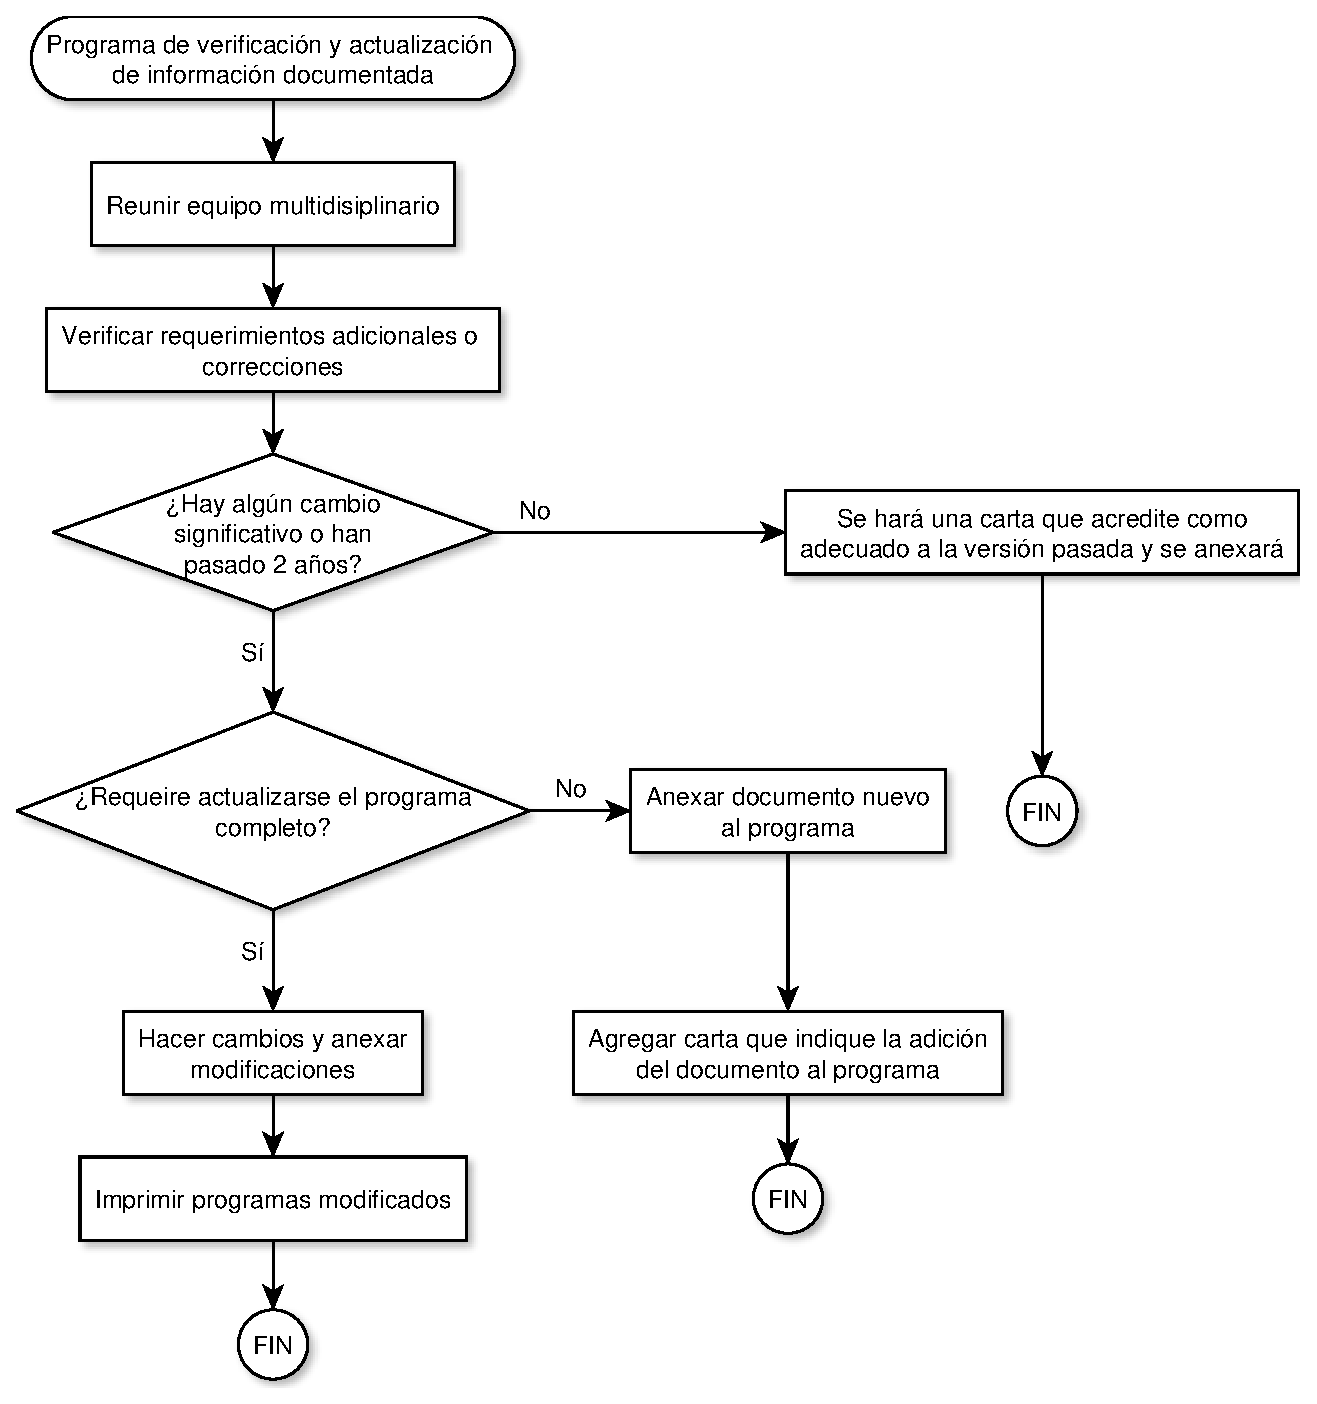
\includegraphics[width=0.5\linewidth]{src/diagramas/G1_AV1.eps}
    \caption{Diagrama de flujo del proceso para verificar y/o actualizar \gls{informacion-documentada}.}
\end{figure}

\subsubsection{Revisión de la información documentada}
\index{Información documentada!revisión}
\label{documentacion:revision}
\begin{itemize}
\item Se tienen que evaluar anualmente los programas de \GLS{RDF} con el propósito de determinar áreas de oportunidad. Esto tiene que hacerse con ayuda de un equipo multidisciplinar constituido por administradores de las áreas operativas pertinentes a la \gls{informacion-documentada} que se va a validar;
\item en caso de que se considere adecuada la información establecida en la \gls{informacion-documentada} analizada, se hará una carta que acredite como vigente el programa (ver \cref{documentacion:validacion}).
\end{itemize}

\subsubsection{Validación de la información documental}
\index{Información documentada!validación}
\label{documentacion:validacion}
Una vez revisada la información documental de los programas pertinentes, si se acuerda que la información contenida sigue vigente se tiene que hacer el siguiente procedimiento:
\begin{itemize}
    \item Revisar programas e \gls{informacion-documentada} asociada con ayuda de un equipo multidisciplinar;
    \item elaborar una carta membretada que acredite como \emph{vigente} el programa y se establezca una fecha de revisión futura;
    \item se debe de firmar la carta por el gerente de almacén y por el jefe de aseguramiento de calidad;
    \item en caso de que se tenga que hacer algún \textit{addendum} que no involucre una reestructuración completa del contenido o de la serialización de los documentos; él ---o los--- documentos nuevos deberán agregarse a la carpeta del programa al que pertenece y se agregará una carta membretada que documente las modificaciones o \textit{addendums} al programa. Esta carta debe de firmarse por el gerente de almacén y por el jefe de aseguramiento de calidad.
\end{itemize}

\subsubsection{Formación del equipo multidisciplinar}
\index{Información documentada!equipo multidisciplinar, formación de}
\label{documentacion:formacionEquipo}
La función de tener una reunión con un \emph{equipo multidisciplinar} es el poder determinar que carencias existen en los programas que cada área operativa utiliza.

Para la formación del equipo se debe de considerar lo siguiente:
\begin{itemize}
    \item No es necesario mantener una lista del equipo multidisciplinar estática;
    \item no se requiere forzosamente que se parte del equipo el jefe de cada área, puede pertenecer a la junta cualquier empleado del área operativa;
    \item se tiene que definir el alcance de la junta y el tiempo que se dedicará;
    \item pueden conducirse entrevistas para determinar carencias en el SGC.
    \item no se requiere documentar la minuta de esta reunión, pero sí se requiere elaborar la \emph{carta de vigencia de programa} (ver \cref{documentacion:validacion,carta.validación}).
\end{itemize}


\subsection{Frecuencia}
\index{Información documentada!frecuencia de revisión y validación}

\begin{table}[h]
    \centering
\begin{talltblr}[%
        caption = {Frecuencia de los procesos asociados con la actualización de \gls{informacion-documentada}.},
        label = {freq.act},
        note{$\dag$} = {Puede ser, por ejemplo, la inclusión de un nuevo formulario, procedimiento, instrucción de trabajo, ayuda visual, etc\dots}
        ]
        {%
        colspec = {X[c]X[c]},
        width = 0.6\linewidth,
        }
        \toprule
        Proceso                                                  & Frecuencia                                                                                          \\
        \midrule
        Validación de la \gls{informacion-documentada}                 & Anualmente                                                                                          \\
        Actualización completa de la \gls{informacion-documentada}     & Cada que se haga un cambió considerable o cuando existan cambios en la estructura de los documentos \\
        Generación de carta aprobativa de información documental & Cada que se tenga que hacer un addendum minúsculo a un programa\TblrNote{$\dag$}                    \\
        \bottomrule
\end{talltblr}
\end{table}

\subsection{Responsabilidades}
\index{Información documentada!responsabilidades}
\begin{itemize}
    \item \textbf{Aseguramiento de calidad:} se encarga de producir los cambios al programa;
    \item \textbf{Equipo multidisciplinar:} se encargará de determinar los cambios y adiciones a los programas establecidos;
    \item \textbf{Gerente de almacén:} verificación de las modificaciones y aprobación.
\end{itemize}

\subsection{Acciones preventivas}
\index{Información documentada!acciones preventivas}
\begin{itemize}
    \item Se coordinará con el \emph{equipo multidisciplinar} una fecha para la junta con anticipación suficiente.
\end{itemize}

\subsection{Acciones inmediatas}
\index{Información documentada!acciones inmediatas}
En caso de que no se haya conducido la actualización completa o la verificación de la información documental no será requerido elaborar un estudio de causa raíz, ya que esto no se considera un problema a la inocuidad de los alimentos, sin embargo se procederá a hacer las siguientes acciones inmediatas.

\subsubsection*{En caso de que la junta no se pudiera acordar}
\index{Información documentada!acciones inmediatas!junta no concretada}
\begin{itemize}
    \item Se coordinará con el \emph{equipo multidisciplinar} una fecha diferente para la junta con anticipación suficiente.
\end{itemize}

\subsubsection*{En caso de que las actualizaciones no se hayan concretado en el periodo establecido}
\index{Información documentada!acciones inmediatas!actualización en proceso}
\begin{itemize}
    \item Se seguirá utilizado la \gls{informacion-documentada} anterior hasta que se logren publicar las modificaciones.
\end{itemize}

\begin{changelog}[simple, sectioncmd=\subsection*,label=changelog-1.0]
    \begin{version}[v=1.0, date=2023--01, author=Pablo E. Alanis]
        \item Primera edición.
    \end{version}
\end{changelog} %TODO Acomodar correctamente
\appendix
\pagestyle{formato-PI}
\renewcommand{\MayorVer}{1}
\renewcommand{\MenorVer}{0}
\renewcommand{\Codigo}{BPD-AP-A}
\renewcommand{\FechaPub}{2023--01}
\renewcommand{\Titulo}{Carta de amonestacion}

\section{\Titulo}
\label{AP1}
\begin{figure}[H]
	\centering
	\fbox{%
	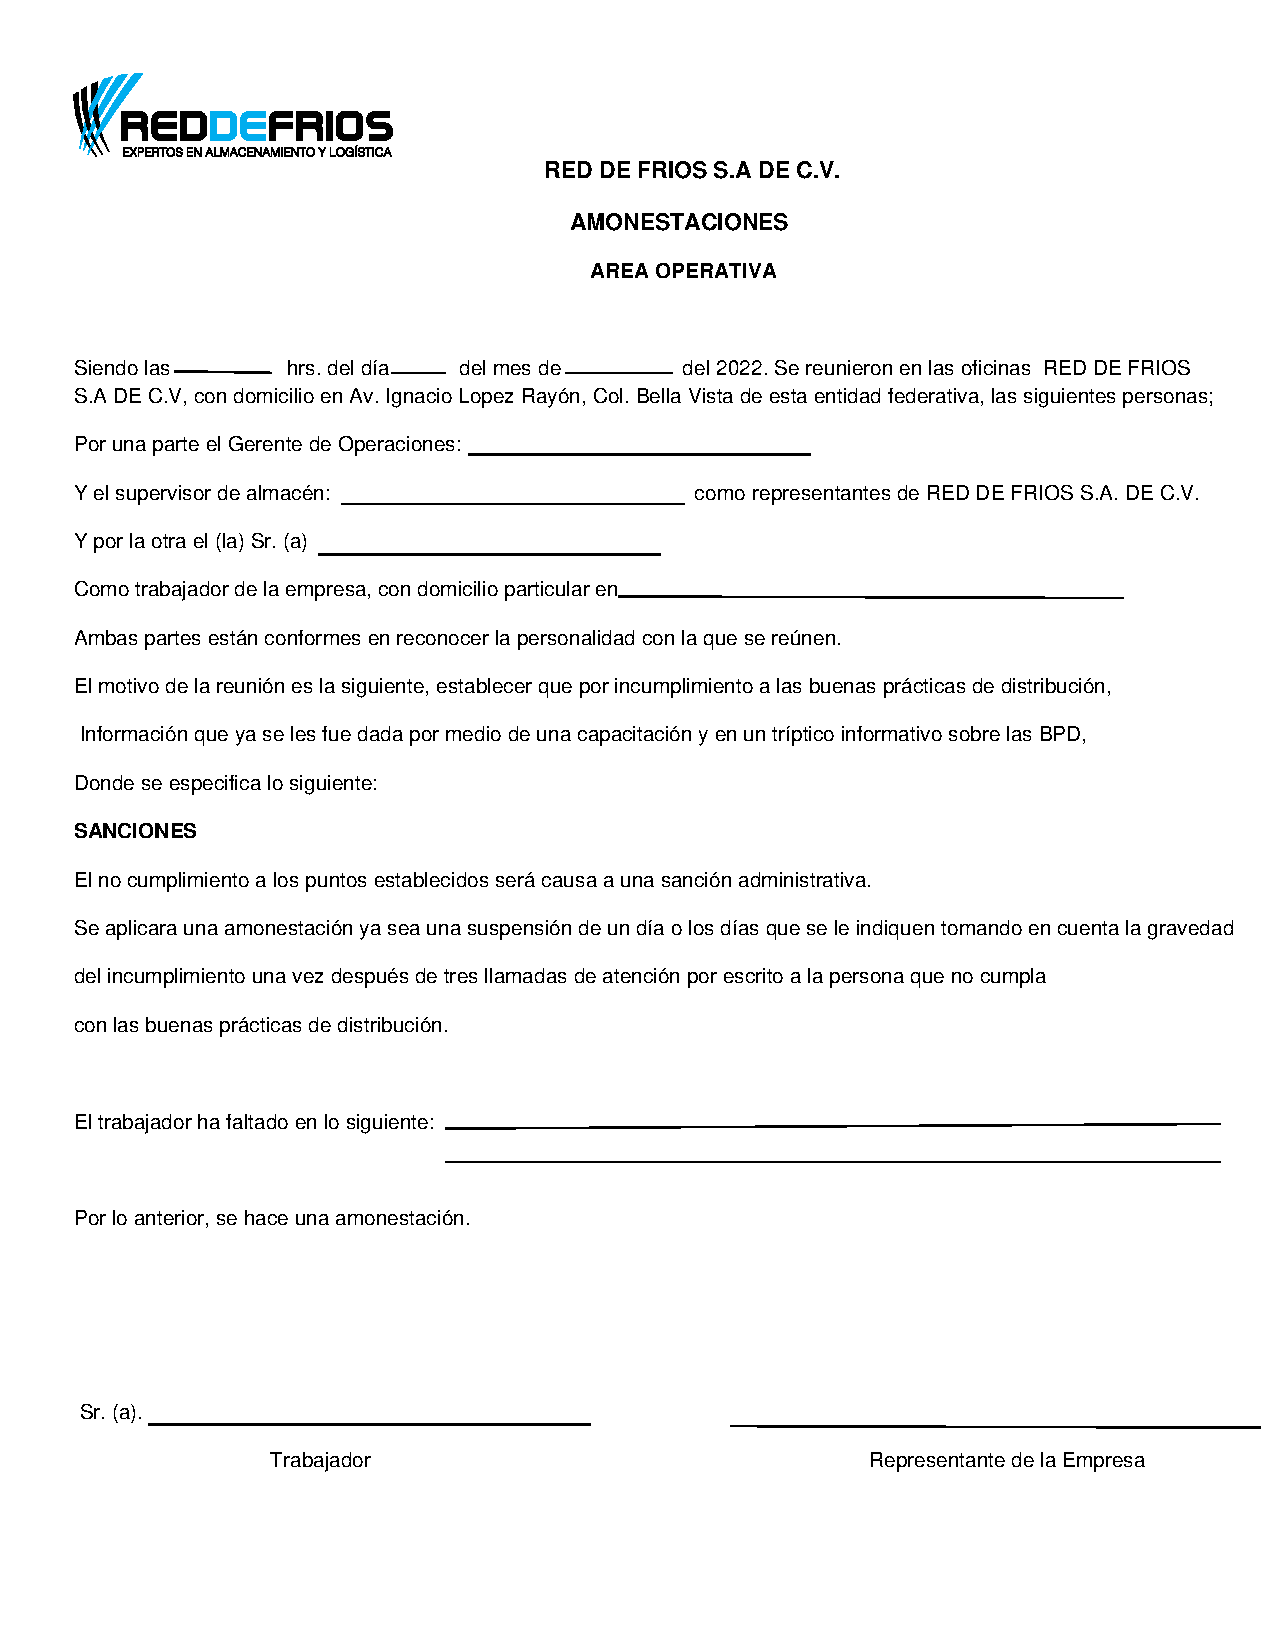
\includegraphics[width=0.70\linewidth]{ref/EXP-Amonestaci.pdf}
	}%
    \label{F-amonest}
	\caption{Formulario de amonestación.}
\end{figure}
\renewcommand{\MayorVer}{1}
\renewcommand{\MenorVer}{0}
\renewcommand{\Codigo}{BPD-A-2}
\renewcommand{\FechaPub}{2023--01}
\renewcommand{\Titulo}{Carta compromiso de cumplimiento del reglamento interno}

\section{\Titulo}
\label{carta.compromiso}
%\section{Reglamento de ingreso a las instalaciones}

\noindent \textit{A quien corresponda,}\bigskip

Se le exhorta a cualquier \emph{personal contratado por clientes de RDF (PCPC)} y \emph{visitante} que se apegue al reglamento de ingreso al almacén descrito abajo \textit{(vide infra).} Con el propósito de resguardar la inocuidad de los productos alimenticios aquí almacenados, así como para prevenir incidentes dentro del área operativa.
\vspace{2\baselineskip}
\begin{center}
    \fbox{%
        \begin{minipage}{0.9\linewidth}
            \small
            \begin{itemize}
                \item Se deben de lavar las manos al entrar al área operativa con jabón y gel antibacteriano;\footnote{En caso de portar guantes, estos deberán estar limpios y de todas maneras, el procedimiento de lavado y desinfección de manos adecuado deberá ser realizado.}
                \item Traer su uniforme completo;
                \item Prohibido portar joyería;\footnote{\textit{i.e.} Anillos, cadenas, aretes, pulseras, piercings en lugares visibles.}
                \item Prohibido fumar;
                \item Prohibido masticar chicle;
                \item Prohibido comer o beber en las áreas operativas;
                \item Prohibido escupir;
                \item Usar ropa y/o uniforme limpio;
                \item Prohibido usar pantalones deshilachados o con pedrería;
                \item Prohibido entrar en shorts y camisas sin mangas;
                \item Usar cofias en áreas de dentro de Almacén;
                \item Usar cubrebocas en el Almacén;
                \item No portar artículos en bolsillos superiores a la cintura;
                \item Prohibido introducir artículos de vidrio;
                \item No golpear ni dañar los productos;
                \item Mantener limpias y en orden las áreas y las herramientas de trabajo;
                \item Prohibido el uso de  calzado abierto;
                \item No pisar los productos ni las tarimas;
                \item No colocar en el piso material de contacto con producto \emph{i.e.} emplayes, cajas de plástico, etc.;
                \item No utilizar celulares personales dentro del almacén;\footnote{Si se tiene que utilizar el celular para una cuestión que involucre la operación, el personal que lo haya usado tendrá que lavarse y desinfectarse las manos nuevamente antes de tocar cualquier producto alimenticio.}
                \item Traer las uñas de las manos cortas;
                \item Prohibido usar barba larga;
                \item Si se tiene el cabello largo, este debe de estar completamente cubierto por la cofia;
                \item Prohibido el uso de cámara fotográfica y de video de cualquier tipo dentro del almacén sin autorización previa.
            \end{itemize}
        \end{minipage}
    }%
\end{center}

\vfill
\begin{center}
\noindent\begin{tabular}{@{}>{\centering}p{2.5in}>{\centering}p{2.5in}@{}}
    \small
    \hrulefill                         & \hrulefill \tabularnewline
    \textbf{\textit{Nombre del PCPC o visitante\\y empresa en que labora}}      & \textbf{\textit{Firma}}\\  
    \end{tabular}
\end{center}
\vfill

\renewcommand{\MayorVer}{1}
\renewcommand{\MenorVer}{0}
\renewcommand{\Codigo}{BPD-AP-C}
\renewcommand{\FechaPub}{2023--01}
\renewcommand{\Titulo}{Carta de validación de información documentada}

\section{\Titulo}
\label{carta.validación}

\noindent\makebox[\textwidth][c]{%
\fbox{%
\begin{minipage}[H]{0.8\linewidth}


\includegraphics[width=0.4\textwidth]{RDF_Logo.png} % Logo

\vspace{1em} % Pull the rule closer to the logo

\rule{\linewidth}{1pt} % Horizontal rule

\bigskip\bigskip % Vertical whitespace

\hfill
\begin{tabular}{l @{}}
	\framebox[4cm][c]{\textit{Fecha}} \bigskip\\ % Date
	Red de Fríos S.A. de C.V. \\
    \\ % Address
    Ignacio López Rayón No. 2810 N, \\
    Col. Bellavista, C.P. 64410, Monterrey, NL, México   \\
	Teléfono: (+52) 81 8351-0512 \\
	www.reddefrios.com.mx
\end{tabular}

\bigskip % Vertical whitespace

    \noindent \textit{A quien corresponda,} \bigskip

Con base en los hallazgos tras evaluar los requerimientos del sistema de gestión de calidad, el equipo multidisciplinario compuesto por \framebox[5cm][c]{\textit{indicar nombres}} ha acordado que los contenidos del programa \framebox[5cm][c]{\textit{indicar programa}} podrá seguir vigente hasta \framebox[5cm][c]{\textit{indicar fecha de vencimiento}}.\par

\vspace{1.5\baselineskip} \ \\
 
\noindent En caso de hacer \textit{addendums,} estos se harán sobre el programa actual, sin necesidad de modificar la estructura del mismo.

\vspace{5cm}

\begin{center}
\noindent\begin{tabular}{@{}>{\centering}p{2.5in}>{\centering}p{2.5in}@{}}
    \small
    \hrulefill                         & \hrulefill \tabularnewline
    \textbf{\textit{Jefe de aseguramiento de calidad}}      & \textbf{\textit{Gerente de almacén}}\\  
    \end{tabular}
\end{center}

\vfill

\end{minipage}
}}
\renewcommand{\MayorVer}{1}
\renewcommand{\MenorVer}{0}
\renewcommand{\Codigo}{BPD-GLOS}
\renewcommand{\FechaPub}{2023--01}
%\renewcommand{\Edit}{01}
\renewcommand{\Titulo}{Programa de Buenas Prácticas de Distribución --- Glosario}
\printglossary
\renewcommand{\MayorVer}{1}
\renewcommand{\MenorVer}{0}
\renewcommand{\Codigo}{BPD-IND}
\renewcommand{\FechaPub}{2023--01}
%\renewcommand{\Edit}{01}
\renewcommand{\Titulo}{Programa de Buenas Prácticas de Distribución --- Indice alfabético}
\printindex
\end{document}